% Relatório da versão 1 do software ipump para o curso
% Sistemas de Controle - DCA0206 - UFRN
% Autores:
%   AUGUSTO MATHEUS PINHEIRO DAMASCENO
%   MARCEL DA CÂMARA RIBEIRO DANTAS
%   PABLO HOLANDA CARDOSO
%   PEDRO DE CASTRO GURGEL LIMA
%   RODRIGO DANTAS DA SILVA
% Modificado por: Ícaro Bezerra Queiroz de Araújo
%

%%%%%%%%%%%% STRUCTURE %%%%%%%%%%%%%%%
\documentclass[a4paper,12pt]{article}
\usepackage[T1]{fontenc}
\usepackage[utf8]{inputenc}
\usepackage[brazil]{babel}
\usepackage{lmodern}
\usepackage{setspace}
\usepackage[top=2cm, bottom=2cm, left=2cm, right=2cm]{geometry}
%%%%%%%%%%%%%%%%%%%%%%%%%%%%%%%%%%%%%%

%%%%%%%%%%%%%%%% PAGES STYLE %%%%%%%%%
\usepackage{fancyhdr}
\fancypagestyle{main}{
\renewcommand{\headrulewidth}{0pt}
\fancyhead[RO]{\thepage}
\fancyfoot[CO]{}
}
%%%%%%%%%%%%%%%%%%%%%%%%%%%%%%%%%%%%%%

\usepackage{graphicx}
\usepackage{float}
\usepackage{epstopdf}
\usepackage{subfig}
\usepackage{mathptmx}
\usepackage{changepage}


\usepackage{listings}
\usepackage{xcolor}
\lstset{language=C++,
                basicstyle=\ttfamily,
                keywordstyle=\color{blue}\ttfamily,
                stringstyle=\color{red}\ttfamily,
                commentstyle=\color{green}\ttfamily,
                morecomment=[l][\color{magenta}]{\#}
}

%\usepackage[alf]{abntex2cite}

%%%%%%%%%%% PDF METADATA %%%%%%%%%%%%%
\usepackage[ pdftitle={MODELO RELATÓRIO},
pdfsubject={INTRODUÇÃO AO LABORATÓRIO DE CONTROLE - Grupo 3},
pdfkeywords={Controle,Automação,UFRN,DCA,ipump},
hidelinks]{hyperref}
%%%%%%%%%%%%%%%%%%%%%%%%%%%%%%%%%%%%%%

\begin{document}

\onehalfspacing

\thispagestyle{empty}

\setcounter{page}{1}

%%%%%%%%%%%% LOGOS %%%%%%%%%%%%%%%%%%%

\begin{figure}[!ht]

\centering

\subfloat{

\includegraphics[width=2.7cm]{UFRN.eps}
\label{UFRN Logo}
}
\hspace{11.09cm}
\subfloat{

\includegraphics[width=2.4cm]{DCA.eps}
\label{DCA Logo}
}

%\caption{}
\label{Logos}

\end{figure}

%%%%%%%%%%%%%%% CAPA %%%%%%%%%%%%%%%%%

\vspace{-1cm}

\begin{center}
{\bf{\normalsize UNIVERSIDADE FEDERAL DO RIO GRANDE DO NORTE\\
CENTRO DE TECNOLOGIA\\
DEPARTAMENTO DE ENGENHARIA DE COMPUTAÇÃO E AUTOMAÇÃO\\
CURSO DE ENGENHARIA DE COMPUTAÇÃO
}}


\vspace{3.6cm}

{\bf{\large RELATÓRIO DA 3ª EXPERIÊNCIA\\
CONTROLE DE SISTEMAS DINÂMICOS: SISTEMA DE SEGUNDA ORDEM\\
}}
\vspace{1.5cm}
{\large TURMA: 01 A\\
	GRUPO Nº}

\vspace{3.6cm}


\begin{flushright}
\begin{normalsize}
ANDRESSA STÉFANY SILVA DE OLIVEIRA: 20160154101\\
\vspace{0.8cm}
FERNANDA MONTEIRO DE ALMEIDA: 20160154228\\
\vspace{0.8cm}
VITOR RAMOS GOMES DA SILVA: 20160154415\\
\vspace{0.8cm}
MÁRCIO LUIZ BEZERRA LOPES JÚNIOR: 20160154326\\
\end{normalsize}
\end{flushright}


\vspace{2.5cm}

{\large Natal-RN\\
2017}

\end{center}

\newpage

%%%%%%%%%%%%%%%  CONTRA-CAPA %%%%%%%%%

\thispagestyle{empty}

\begin{center}
\begin{normalsize}
ANDRESSA STÉFANY SILVA DE OLIVEIRA: 2016015410\\
\vspace{0.8cm}
FERNANDA MONTEIRO DE ALMEIDA 20160154228\\
\vspace{0.8cm}
VITOR RAMOS GOMES DA SILVA: 20160154415\\
\vspace{0.8cm}
MÁRCIO LUIZ BEZERRA LOPES JÚNIOR: 20160154326\\

\end{normalsize}
\end{center}
\vspace{3cm}

{\bf{\large {\centering CONTROLE DE SISTEMAS DINÂMICOS: SISTEMA DE SEGUNDA ORDEM\\}}}

\vspace{4cm}

\begin{adjustwidth}{7.5cm}{0cm}

{\normalsize

Terceiro Relatório apresentado à disciplina de
Laboratório de Sistemas de Controle, correspondente à
avaliação da 1º unidade do semestre 2017.1 do 8º período
do curso de Engenharia de Computação da
Universidade Federal do Rio Grande do Norte, sob
orientação do {\bf Prof. Fábio Meneghetti Ugulino de
Araújo.}

}

\end{adjustwidth}

\vspace{2cm}

\begin{center}

Professor:  Fábio Meneghetti Ugulino de Araújo.

\vspace{2.5cm}

{\large Natal-RN\\
2017}

\end{center}

\newpage

%%%%%%%%%%%%%%%  RESUMO %%%%%%%%%%%%%%

\thispagestyle{empty}

\begin{center}
{\large \textbf{RESUMO}}
\end{center}

\vspace{3cm}

\begin{flushleft}

\hspace{4ex}O presente trabalho é uma continuação ao que foi previamente realizado na primeira prática. Consiste no desenvolvimento de um software que se comunica com um sistema de tanques, uma planta Quanser, e seu simulador, com canais para leitura e escrita de sinais. Nesta etapa do trabalho, foi-se adicionado ao software desenvolvido na primeira experiência as ações de controle proporcional (P), integral (I) e derivativo (D), possibilitando ao usuário a opção de escolher entre controladores P, PI, PD, PID e PI-D. As funções teóricas utilizadas para formular o controlador estão explicitadas no texto deste relatório, bem como os algoritmos que simulam seus funcionamentos. O comportamento do sistema pode ser observado pelo usuário através de três gráficos presentes na interface do software, um para o sinal de entrada e os demais para os canais de saída.\\

\end{flushleft}

\vspace{1.5cm}

\textbf{Palavras-chave:} sistema de tanques; sistema de controle; software; planta Quanser, controlador PID.

\newpage

%%%%%%%%% LISTA DE FIGURAS %%%%%%%%%%%

\thispagestyle{empty}

\begin{center}
\listoffigures
\end{center}

\newpage

%%%%%%%%%%%%%%% SUMÁRIO %%%%%%%%%%%%%%

\thispagestyle{empty}

\begin{center}
\tableofcontents
\end{center}

\newpage

%%%%%%%%%%%%%%% INTRODUÇÃO %%%%%%%%%%%

\thispagestyle{main}

\section{INTRODUÇÃO}

\begin{flushleft}
\hspace{4ex}As práticas de laboratório feitas anteriormente tinham o foco no controle da planta \textit{Quanser} visando apenas o tanque de cima, ou seja, utilizando um sistema de primeira ordem. Neste relatório, também será apresentado um controle usando PID, de acordo com a escolha do usuário, porém, o foco será no controle do nível do tanque de baixo, o qual é caracterizado como de segunda ordem.

\hspace{4ex}Assim como anteriormente, o usuário poderá escolher a opção entre malha aberta e malha fechada, o sinal de referência a ser enviado, o offset, como também, o tipo do controlador (P, PI, PD, PID ou PI-D),os ganhos dos controladores Kp, Ki e ou Kd, ou $\tau_i$ e $\tau_d.$ 

\hspace{4ex}Agora, o usuário também poderá escolher qual análise da resposta do sistema será utilizada para o tempo de subida (t$_r$), por exemplo, de 5\% à 95\%, e o tempo de acomodação (t$_s$), para as faixas de 2\%, 5\% e 10\% do degrau. Além, de ser possível saber os valores do t$_r$, t$_s$, tempo de pico (t$_p$) e o sobressinal (Mp) do sistema de segunda ordem.

\hspace{4ex}No relatório é apresentado em que consiste essa dinâmica, como foi a metodologia, os resultados dos testes e suas conclusões.
\end{flushleft}

\newpage

%%%%%%%%%% REFERENCIAL TEÓRICO %%%%%%%

\thispagestyle{main}

\section{REFERENCIAL TEÓRICO}

\subsection{LUGAR GEOMÉTRICO DAS RAÍZES}
\hspace{4ex}Lugar geométrico das raízes é a representação gráfica dos lugares dos pólos e zeros da função de transferência de malha fechada quando os paramêtros da função, também chamado de ganho, são variados de zero a infinito.
 
%\[ \frac{k_m}{A}u(t)= \frac{a\sqrt{2gh(t)}}{A} \]
%\[ u(t)=  \frac{a\sqrt{2gh(t)}}{k_m}\]
Pode se obter esses lugares através da função de transferência de malha fechada do sistema:
\begin{equation}\label{eq:1}
1 + kG(s)H(s) = 0
\end{equation}

\subsection{CONTROLADOR DE TRÊS TERMOS (PID)}
O controlador PID é o mais utilizado na indústria (DorfBishop, 2009) um dos motivos para que isso ocorra é devido a facilidade de ser controlado no local. Além disso, é amplamente discutido na literatura, com várias publicações de ajustes e ajustes finos (Ogata, 2010). PID modificados como o PI-D também é bastante utilizado. Pode também ser usado em situações em que não se conhece a função de transferência sistema e ainda conseguir um bom resultado. Porém há ressalvas e em alguns sistemas pode se não obter um controle ótimo.

O PID tem como função de transferência a seguinte expressão:

\begin{equation}\label{eq:1}
G_c(s) = K_p + \frac{K_I}{s} + K_D s
\end{equation}

Na equação podemos ver três parâmetros. Quando se atribui zero ao parâmetro derivativo, obtém-se o controlador PI, controlador proporcional e integral:  \[K_D = 0 \] 
Logo, \[G_c(s) = K_p + \frac{K_I}{s} \]
Da mesma forma para o parâmetro da integral:
\[K_I = 0 \] 
Tem-se o controlador proporcional derivativo, ou PD: \[G_c(s) = K_p + K_D s \]

\begin{figure}[!h]
\centering
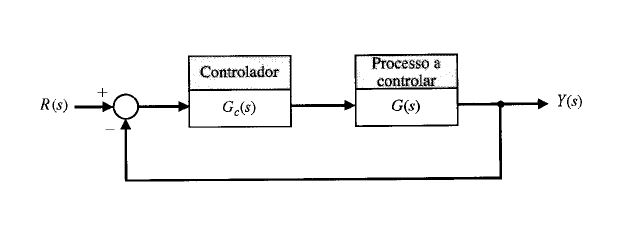
\includegraphics[scale=1]{controlador-malha-fechada.JPG}
\caption{Sistema de malha fechada com controlador}
\label{fig:sistema}
{Fonte: DorfBishop, 2009}
\end{figure}

A função de transferência do PID insere no sistema uma pólo na origem e dois zeros em lugares a serem determinados. Se for adicionado zeros complexos no sistema, têm-se um lugar geométrico das raízes como o exemplo a seguir: 

\begin{figure}[!h]
\centering
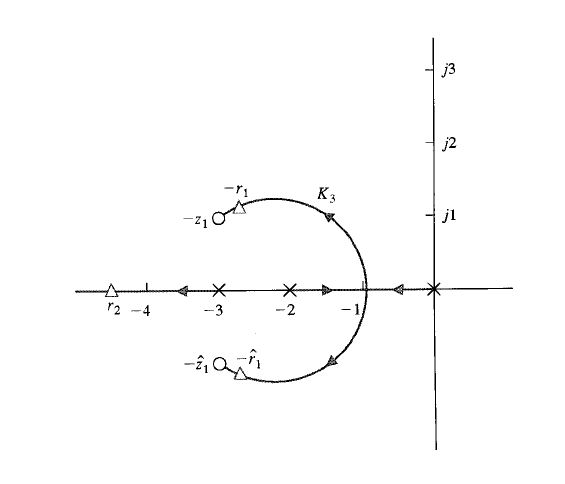
\includegraphics[scale=1]{lugar-das-raizes-pid.JPG}
\caption{Lugar das raízes com zeros complexos}
\label{fig:lgr}
{Fonte: DorfBishop, 2009}
\end{figure}


\subsection{EFEITOS DO CONTROLE DERIVATIVO E INTEGRAL NA PERFORMANCE DO SISTEMA}
\hspace{4ex}
Para um sistema com controle apenas proporcional, dada uma entrada degrau, o erro de regime estacionário aparecerá. Esse offset dependerá do ganho proporcional atribuído. Para que seja eliminado esse erro é necessário a adição de um controlador integral, já que ele adiciona um zero ao sistema, mas pode deixar o sistema mais oscilatório.

Já o controle derivativo quando adicionado a um controle proporcional (PD), oferece um controle com alta sensibilidade, devido a responder a taxa de variação do erro, dessa forma o controle atua antes de forma preventiva (Ogata, 2010). Esse tipo de controle não corrige diretamento o erro de regime estacionário, mas adiciona amortecimento ao sistema de forma que permite um uso de um ganho maior.

Portanto, tendo em mente os efeitos e peculiaridades de cada controlador, pode-se projetar um PID mais eficiente.
\newpage

%%%%%%%%%% METODOLOGIA %%%%%%%%%%%%%%%

\thispagestyle{main}

\section{METODOLOGIA}

\hspace{4ex}O sistema de controle Proporcional Integral Derivativo (PID) desenvolvido foi implementado no código de acordo com o referencial teórico. Para isso, foi criado uma classe que de acordo com a solicitação do usuário será: apenas Proporcional (P), ou Proporcional Integrativo (PI), ou Proporcional Derivativo (PD), ou PID, ou PI-D. A implementação pode ser observada abaixo:

\begin{lstlisting}
double PID::Controle(double e, double h)
{
    I= I+Ki*e*h;
    D= Kd*(e-e_ant)/h;
    e_ant= e;
    return Kp*e+I+D;
}

double PID::Controle(double e, double y, double h)
{
    I= I+Ki*e*h;
    D= Kd*(y-e_ant)/h;
    e_ant= y;
    return Kp*e+I+D;
}
\end{lstlisting}

\hspace{4ex}O primeiro método é referente ao P, PI, PD e PID, enquanto que o segundo método é o PI-D.

\hspace{4ex}Após essa implementação, foram feitos vários testes utilizando todos os tipos de controladores, como também, variando os ganhos.

\newpage

%%%%%%%%%% RESULTADOS %%%%%%%%%%%%%%%

\thispagestyle{main}

\section{RESULTADOS}

\hspace{4ex}Para a análise do comportamento dos controladores foi realizado vários testes diversificando o tipo de controlador e suas variáveis, esses testes podem ser encontrados nos seguintes subtópicos.

\subsection{Controle P}
\hspace{4ex}Utilizando o Controle Proporcional foram obtidos vários resultados variando o valor de Kp, como também o nível desejado, observe a figura \ref{fig:ControleP}.

\hspace{4ex}Notou-se que com o aumento do ganho o sistema se aproxima da referência, mas nunca a alcança. Além disso, a partir de um certo valor de Kp, o sistema começa a ficar instável, como pode ser observado nas figuras \ref{<figureP6>} e \ref{<figureP7>}.
\begin{figure}[H]
     \centering
     \subfloat[][]{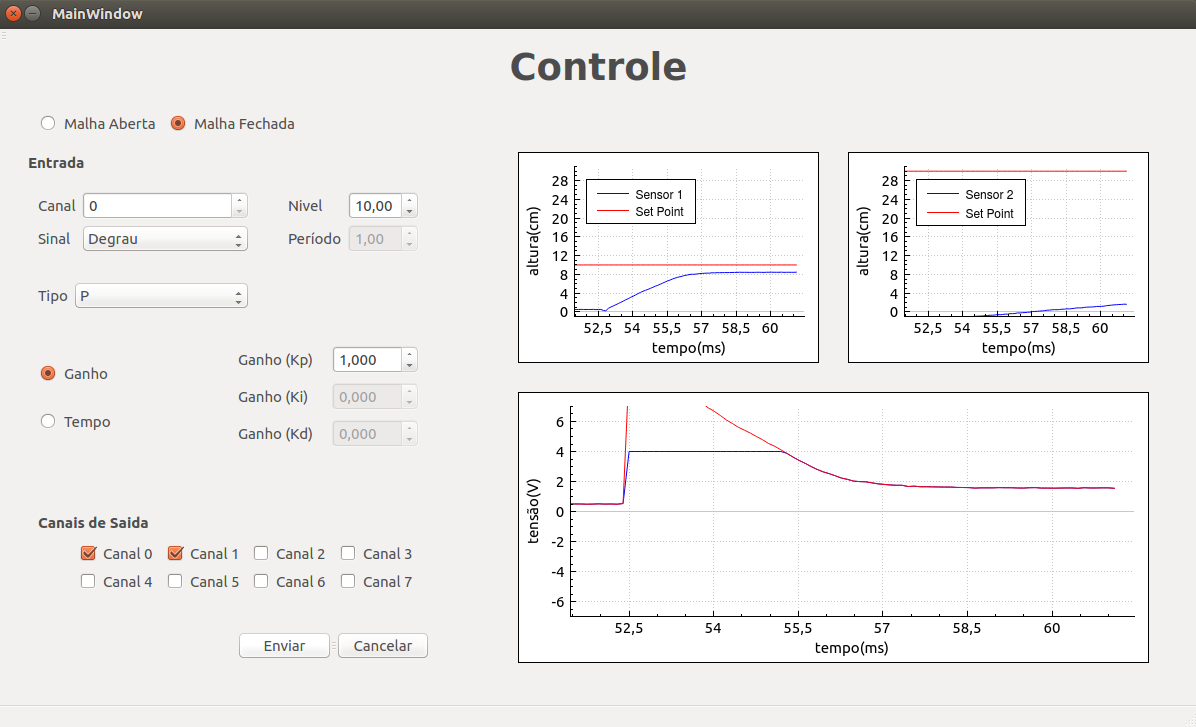
\includegraphics[width=8cm]{resultados/P/00}\label{<figureP1>}}\hspace{4ex}
     \subfloat[][]{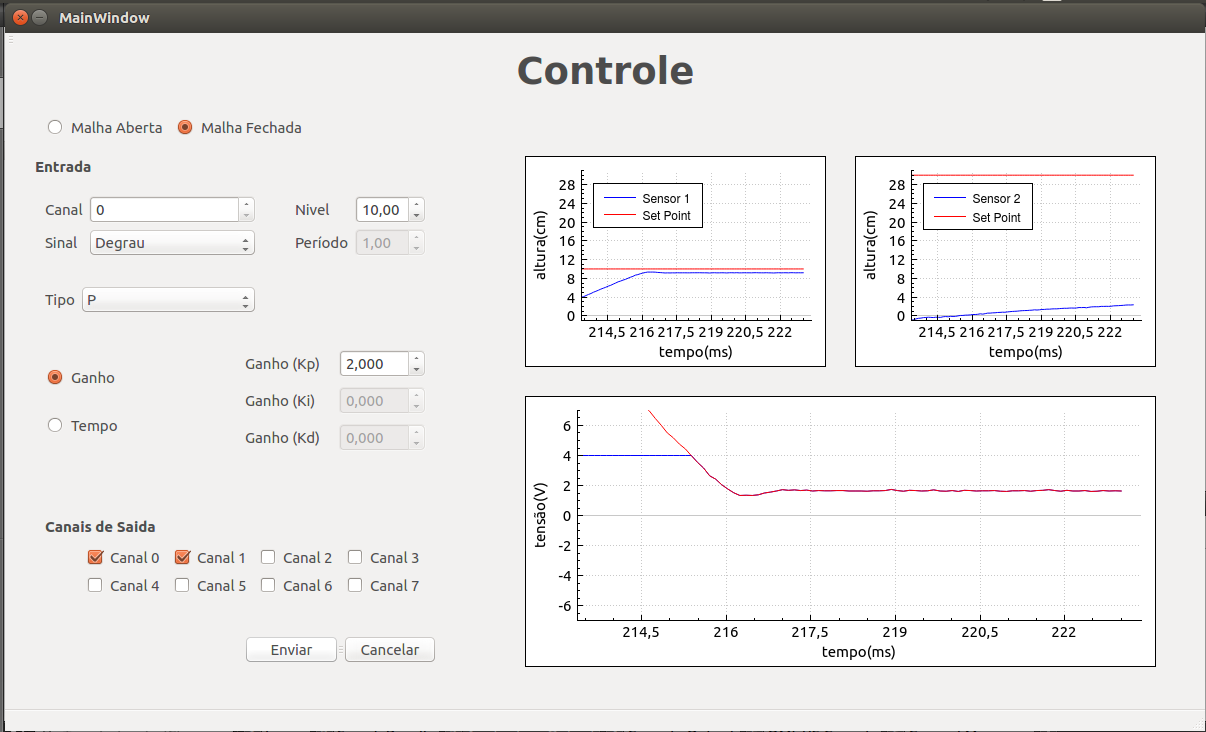
\includegraphics[width=8cm]{resultados/P/01}\label{<figureP2>}}\\
     \subfloat[][]{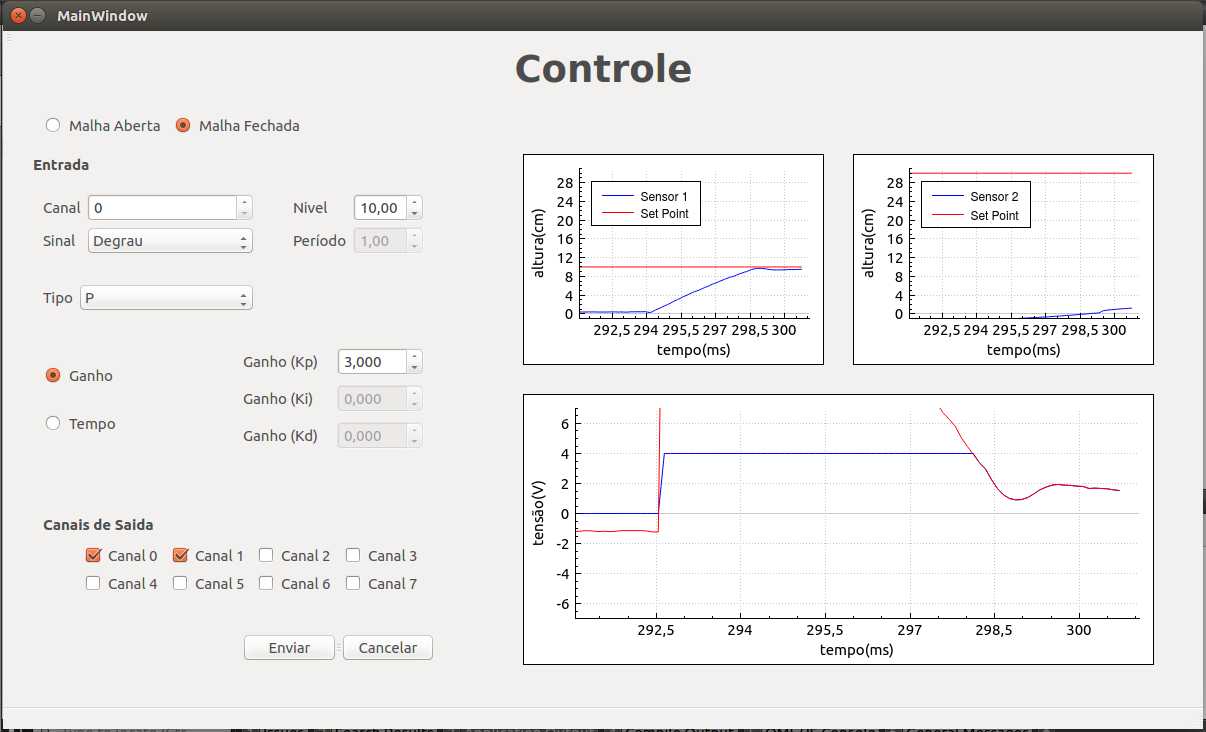
\includegraphics[width=8cm]{resultados/P/02}\label{<figureP3>}}\hspace{4ex}
     \subfloat[][]{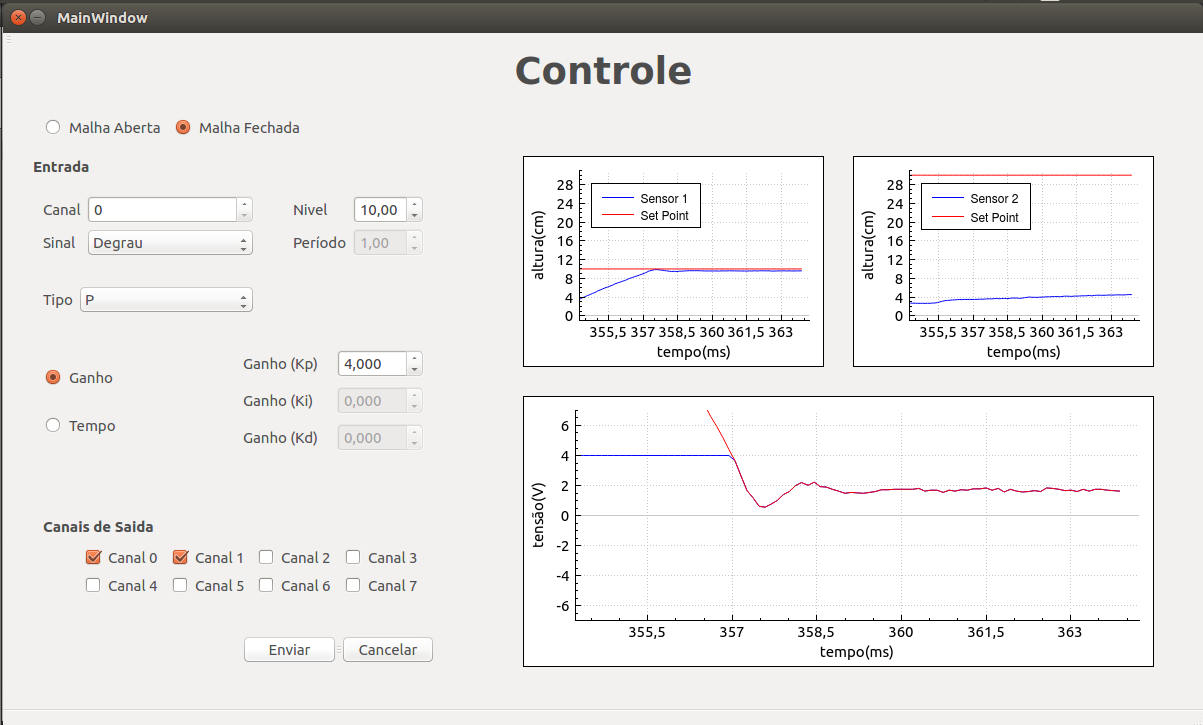
\includegraphics[width=8cm]{resultados/P/03}\label{<figureP4>}}\\
     \subfloat[][]{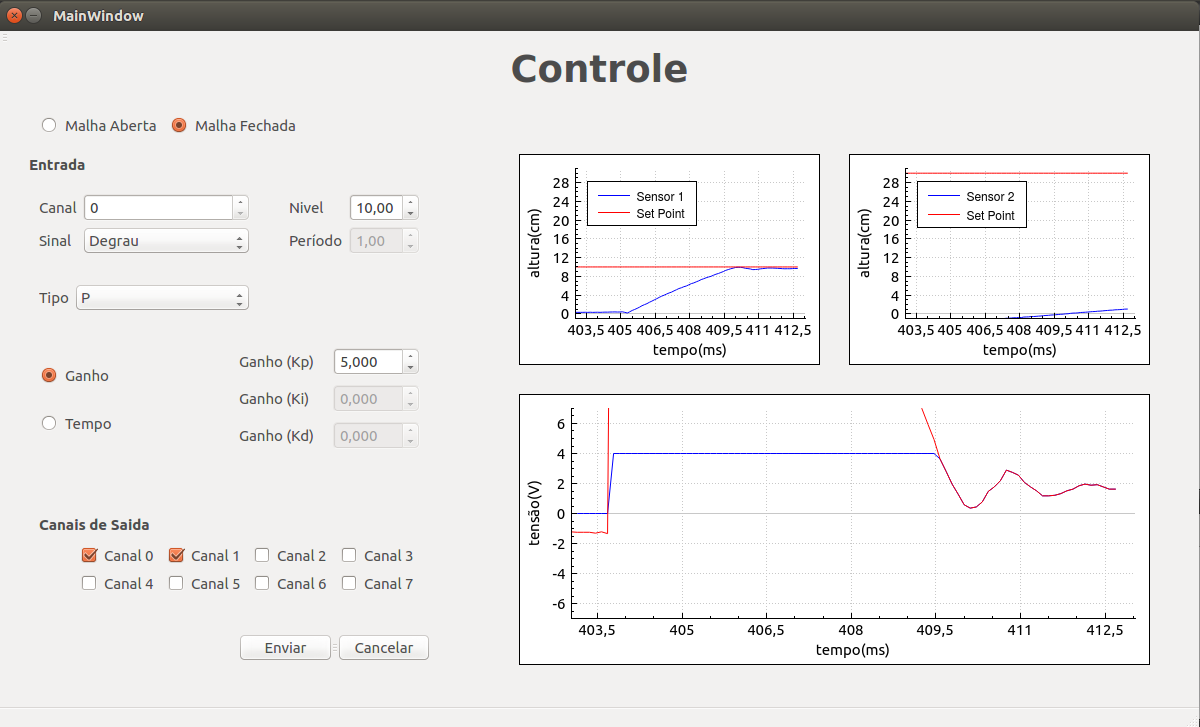
\includegraphics[width=8cm]{resultados/P/04}\label{<figureP5>}}\hspace{4ex}
     \subfloat[][]{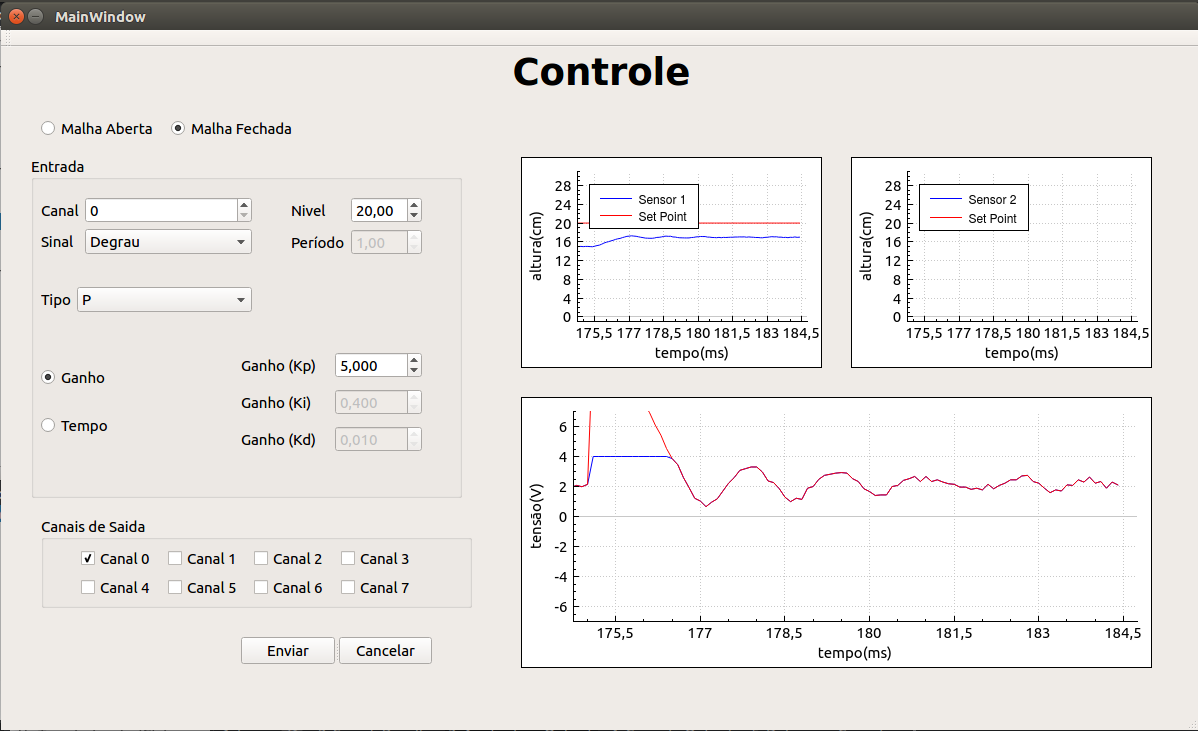
\includegraphics[width=8cm]{resultados/P/05}\label{<figureP6>}}\\
     \subfloat[][]{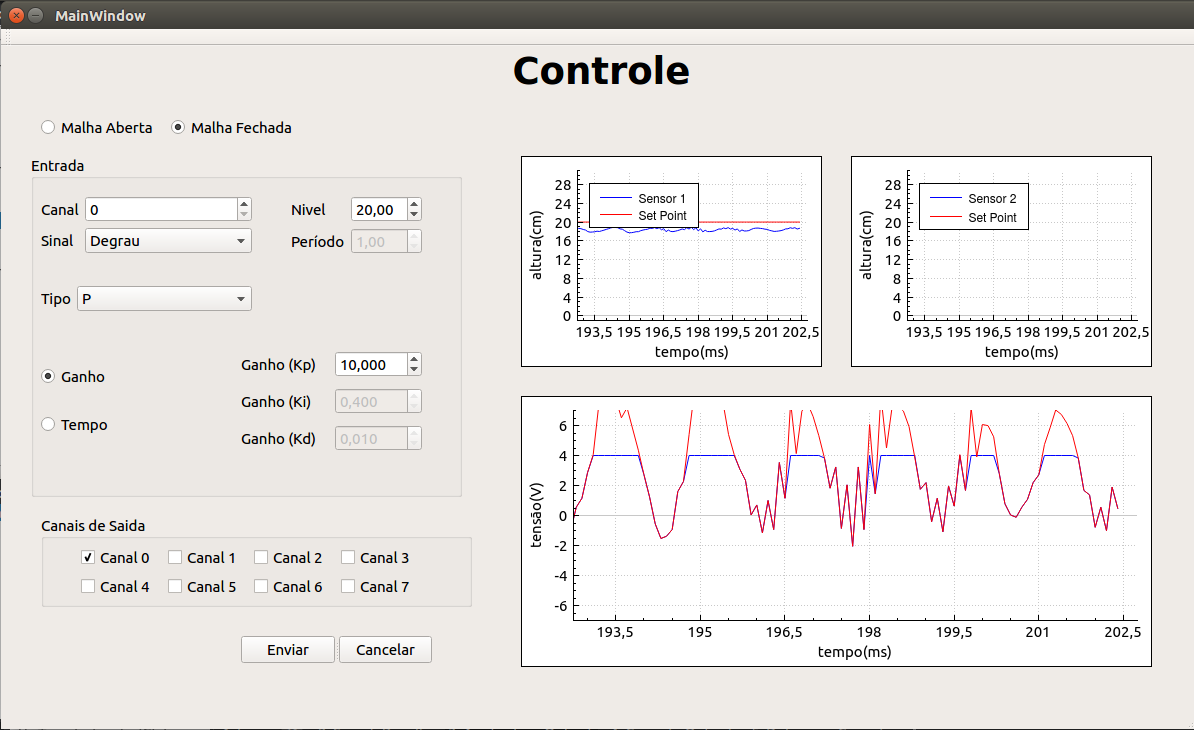
\includegraphics[width=8cm]{resultados/P/06}\label{<figureP7>}}\hspace{4ex}
     \subfloat[][]{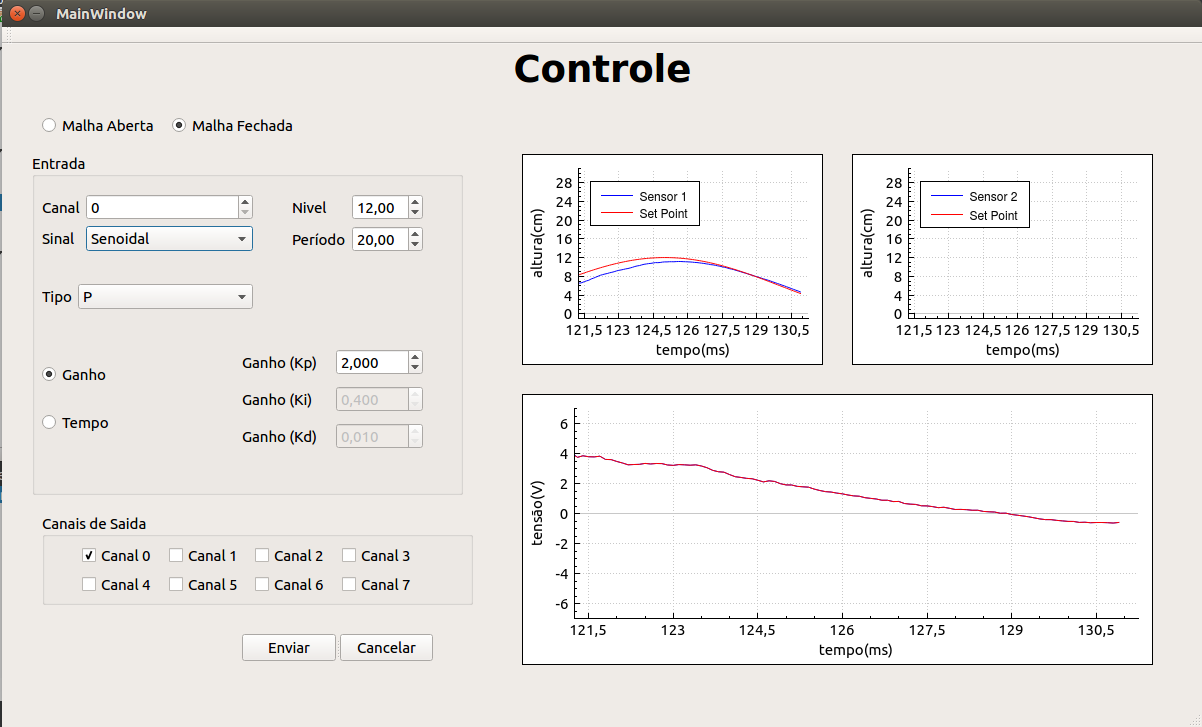
\includegraphics[width=8cm]{resultados/P/07}\label{<figureP8>}}
     \caption{Controle P}
     \label{fig:ControleP}
\end{figure}

\subsection{Controle PI}
\hspace{4ex}Abaixo, na figura \ref{controlePI}, é possível analisar resultados obtidos pela utilização do controle Proporcional Integral.

\hspace{4ex}Como esperado, o nível do tanque consegue atingir o sinal de referência, pois o controlado PI zera o erro de regime para uma entrada degrau.

\hspace{4ex}Também foi verificado que com o aumento do Ki houve um aumento do overshoot, isso pode ser notado nas figuras \ref{<figurePI3>} e \ref{<figurePI4>}.
\begin{figure}[H]
     \centering
     \subfloat[][]{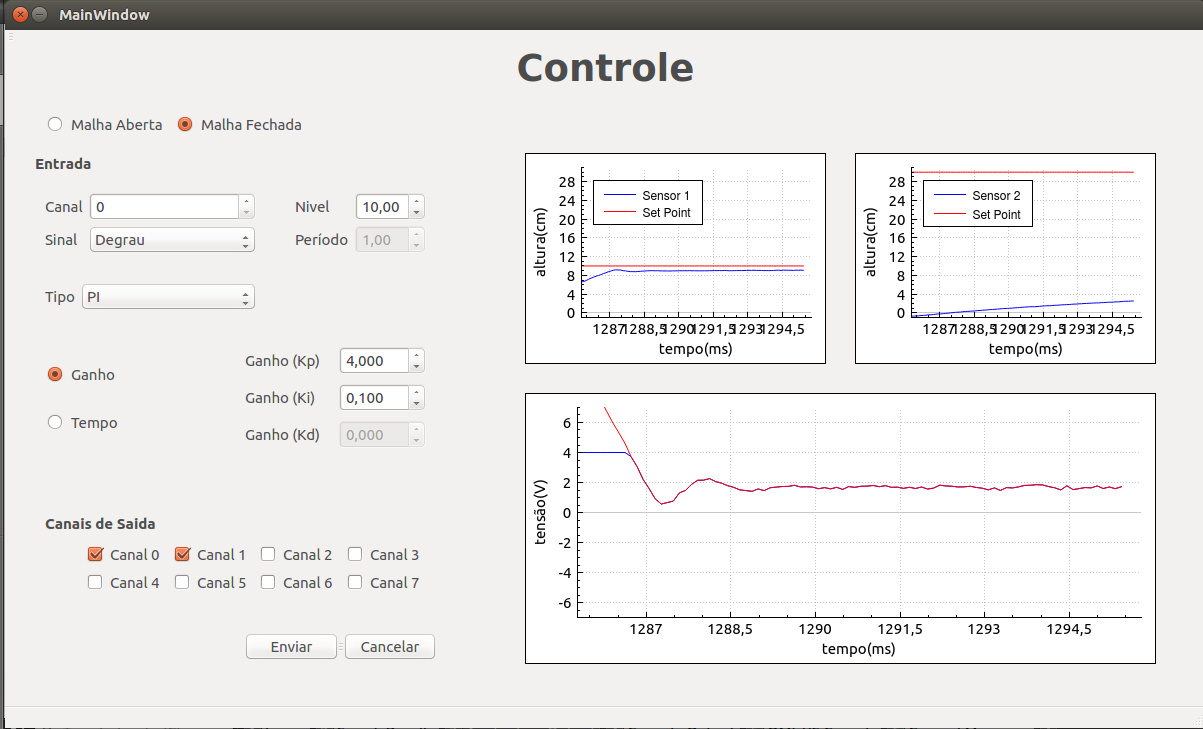
\includegraphics[width=8cm]{resultados/PI/00}\label{<figurePI1>}}\hspace{4ex}
     \subfloat[][]{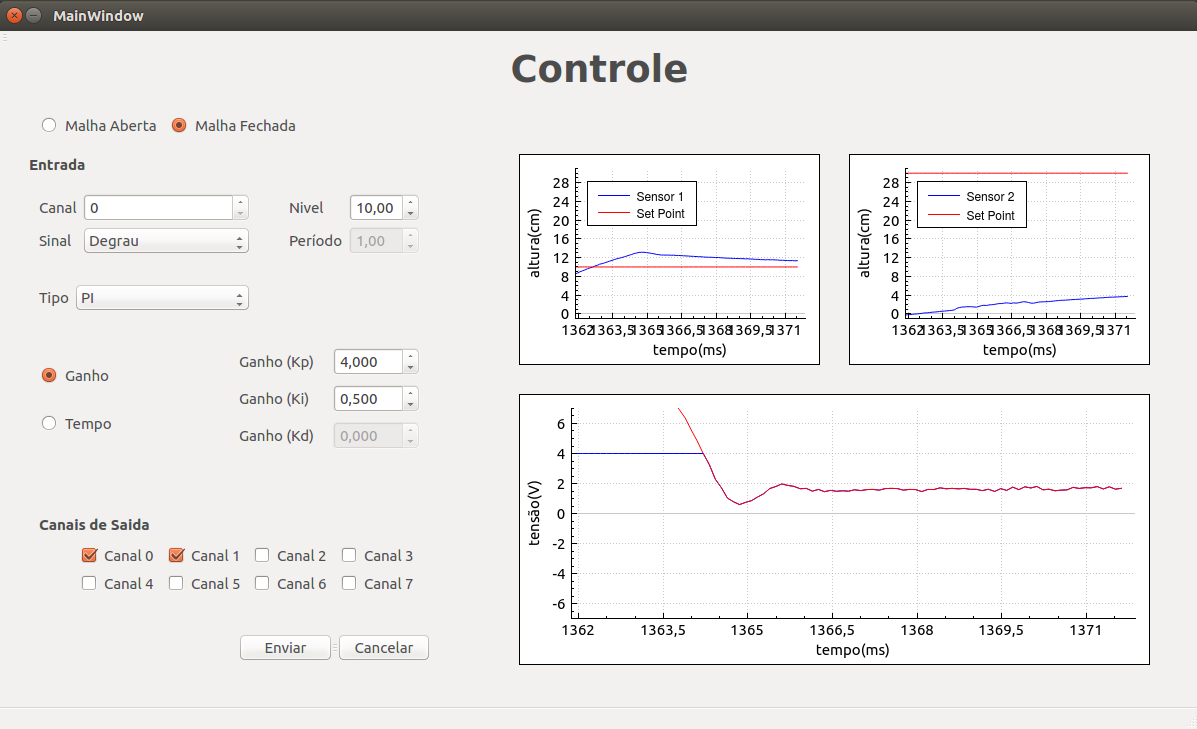
\includegraphics[width=8cm]{resultados/PI/01}\label{<figurePI2>}}\\
     \subfloat[][]{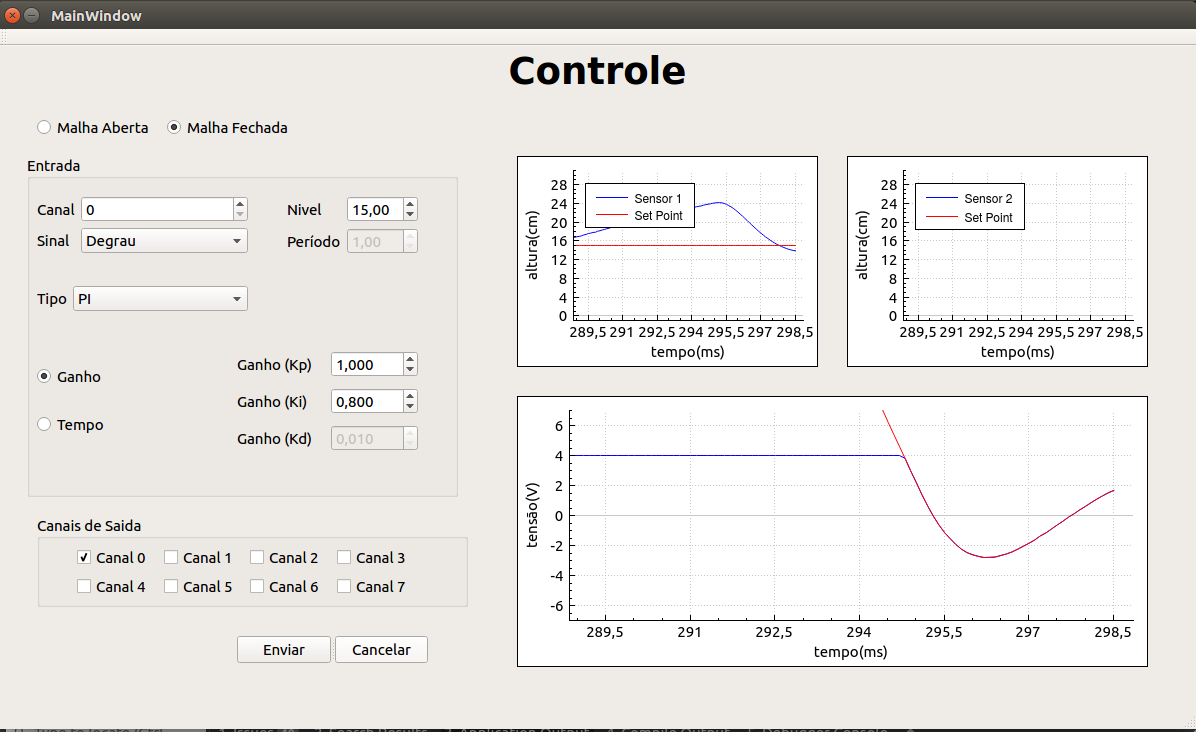
\includegraphics[width=8cm]{resultados/PI/02}\label{<figurePI3>}}\hspace{4ex}
     \subfloat[][]{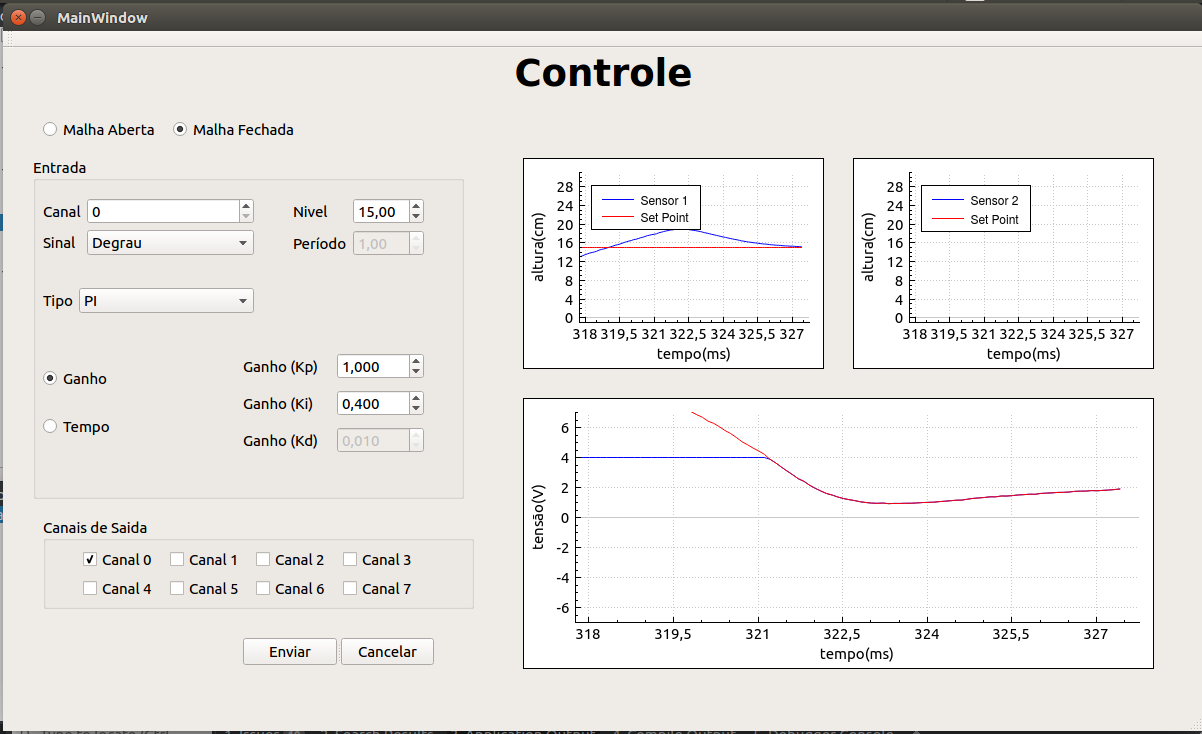
\includegraphics[width=8cm]{resultados/PI/03}\label{<figurePI4>}}\\
     \subfloat[][]{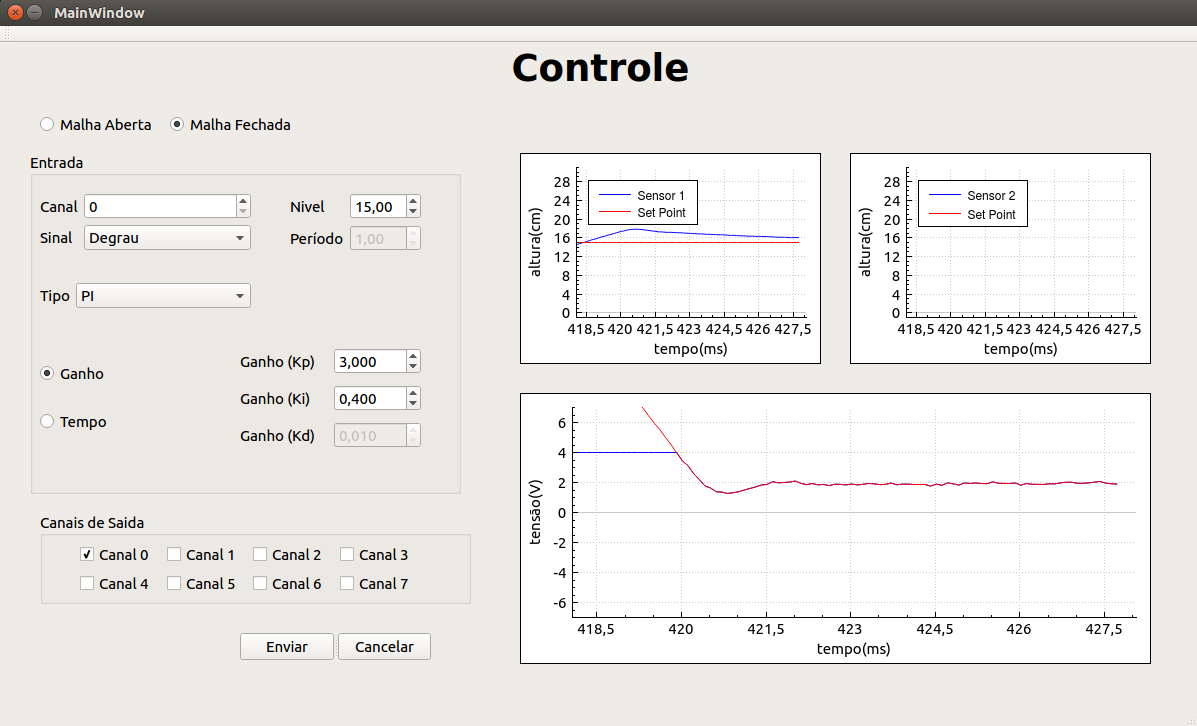
\includegraphics[width=8cm]{resultados/PI/04}\label{<figurePI5>}}\hspace{4ex}
     \subfloat[][]{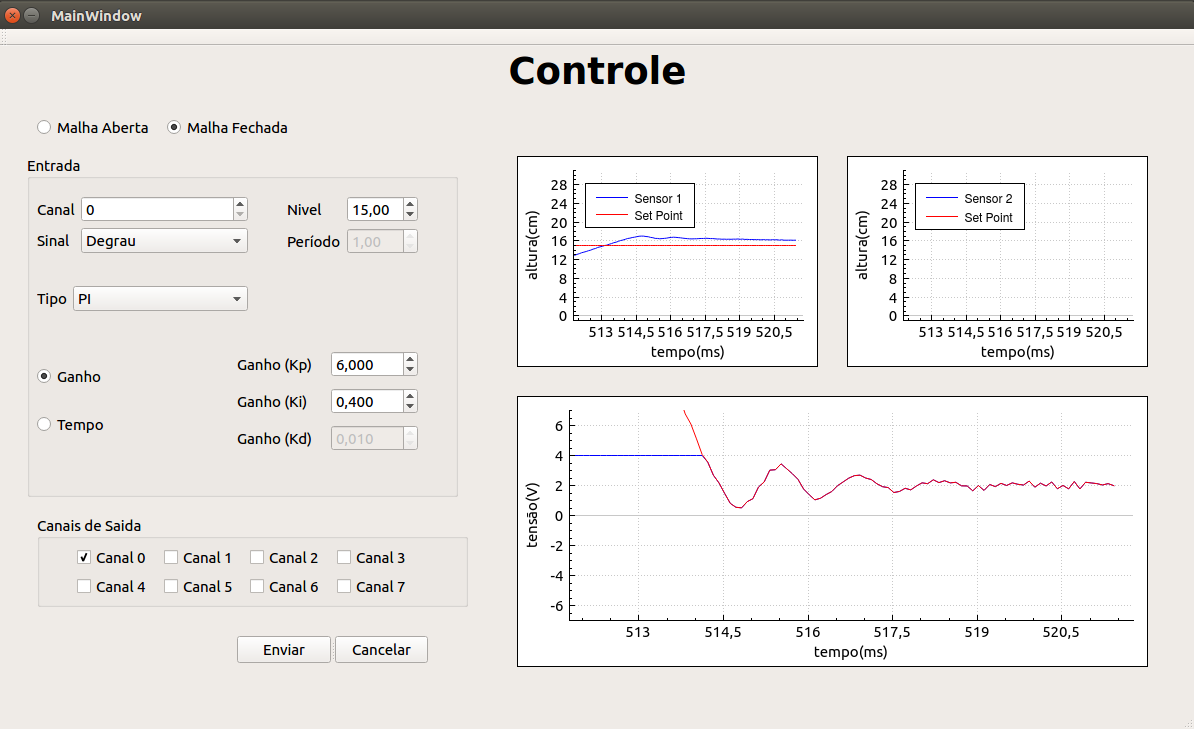
\includegraphics[width=8cm]{resultados/PI/05}\label{<figurePI6>}}\\
     \subfloat[][]{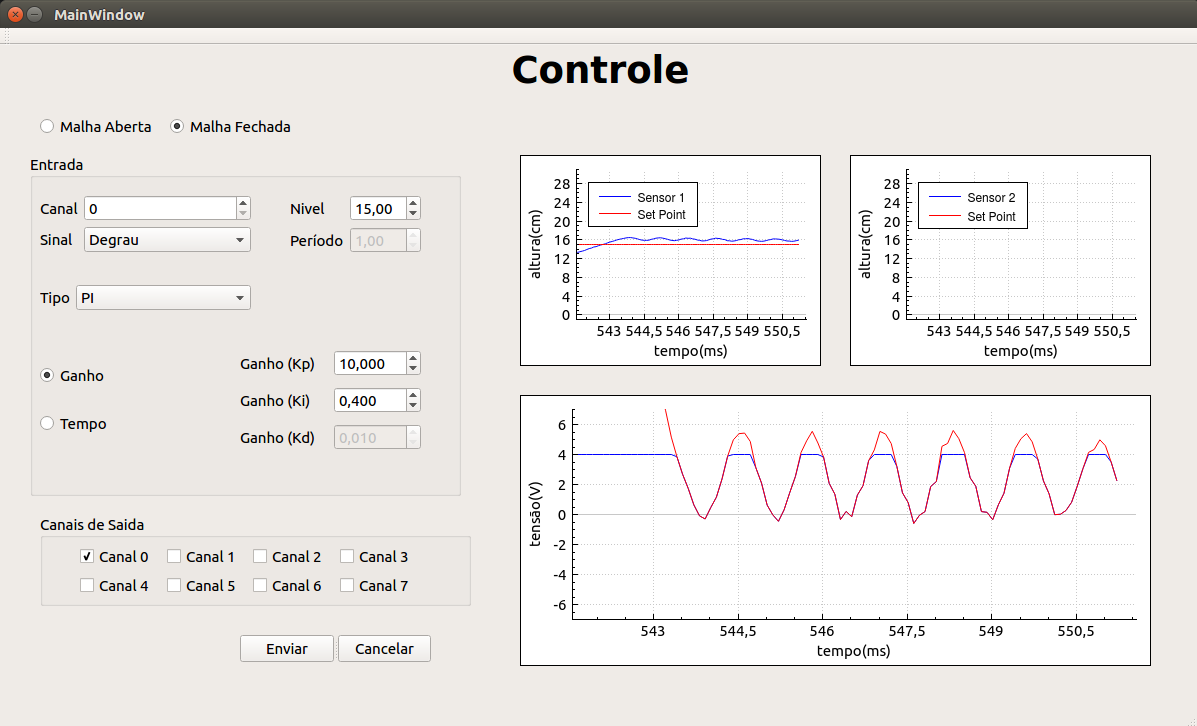
\includegraphics[width=8cm]{resultados/PI/06}\label{<figurePI7>}}
     \caption{Controle PI}
     \label{controlePI}
\end{figure}

\subsection{Controle PD}
\hspace{4ex}O controlador PD tenta prever variações no sinal, dessa forma, melhorando o transitório, veja a figura \ref{controlePD}.

\hspace{4ex}Como também, quando há o aumento do valor do Kd, o sinal de controle fica muito oscilatório como visto na figura \ref{<figurePD4>}.
\begin{figure}[H]
     \centering
     \subfloat[][]{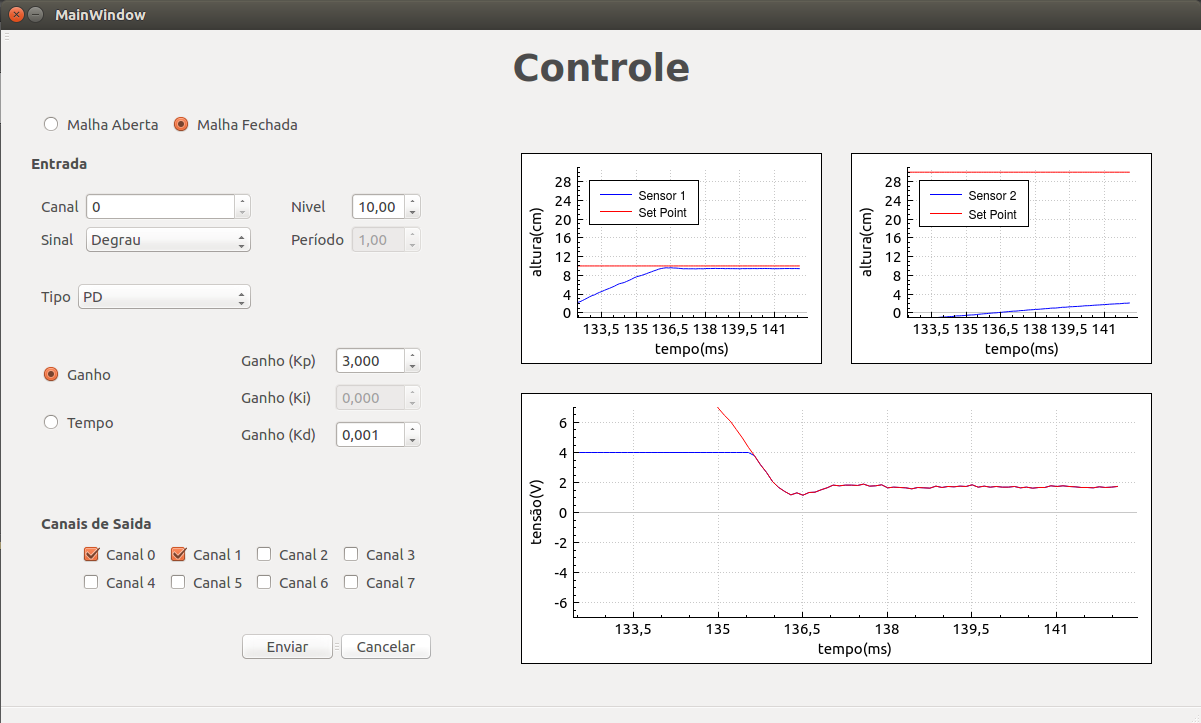
\includegraphics[width=8cm]{resultados/PD/00}\label{<figurePD1>}}\hspace{4ex}
     \subfloat[][]{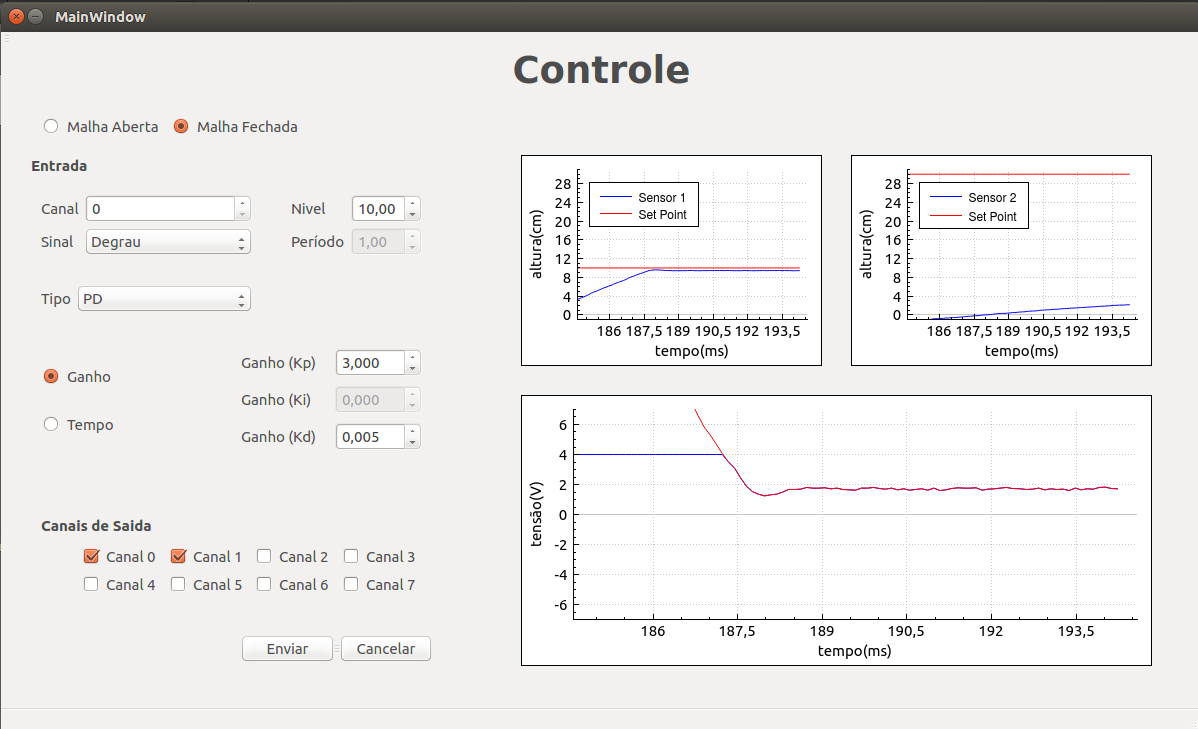
\includegraphics[width=8cm]{resultados/PD/01}\label{<figurePD2>}}\\
     \subfloat[][]{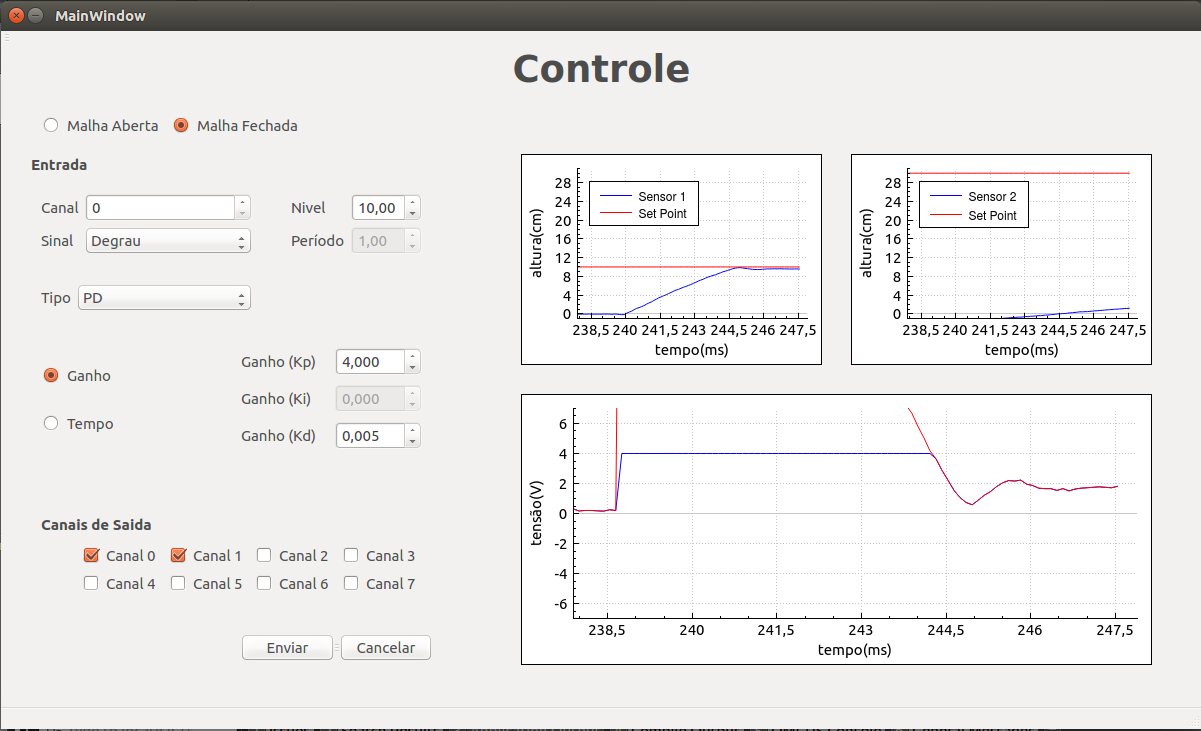
\includegraphics[width=8cm]{resultados/PD/02}\label{<figurePD3>}}\hspace{4ex}
     \subfloat[][]{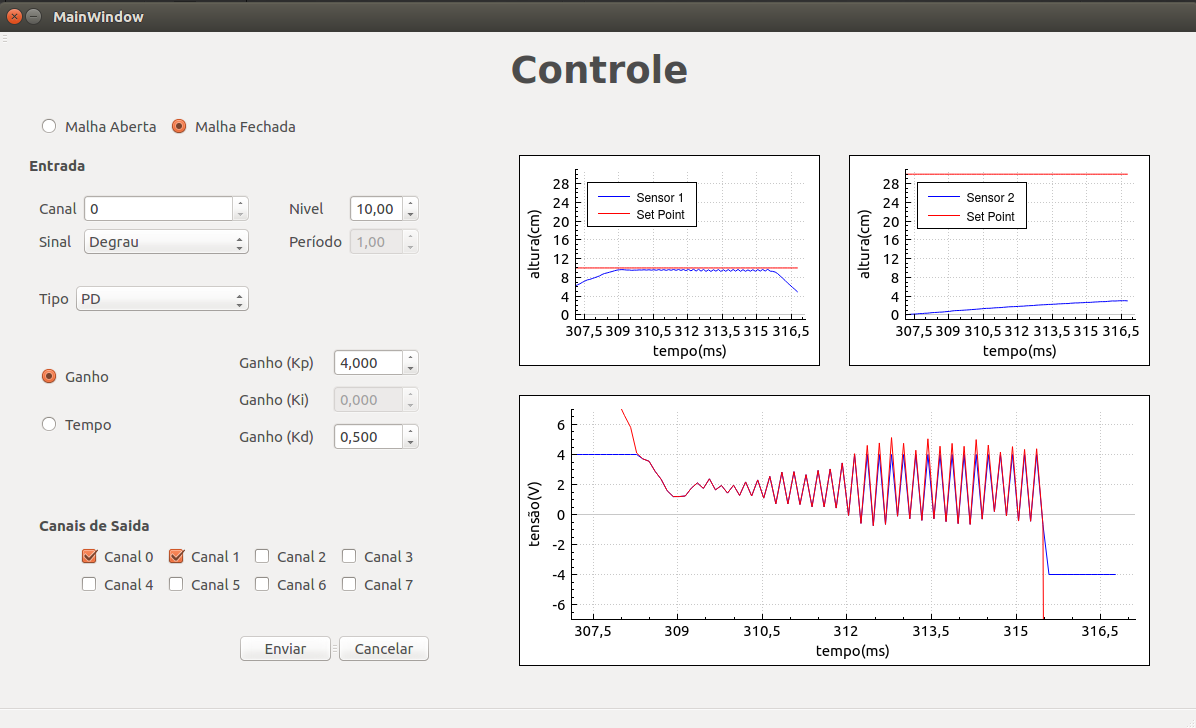
\includegraphics[width=8cm]{resultados/PD/03}\label{<figurePD4>}}\\
     \subfloat[][]{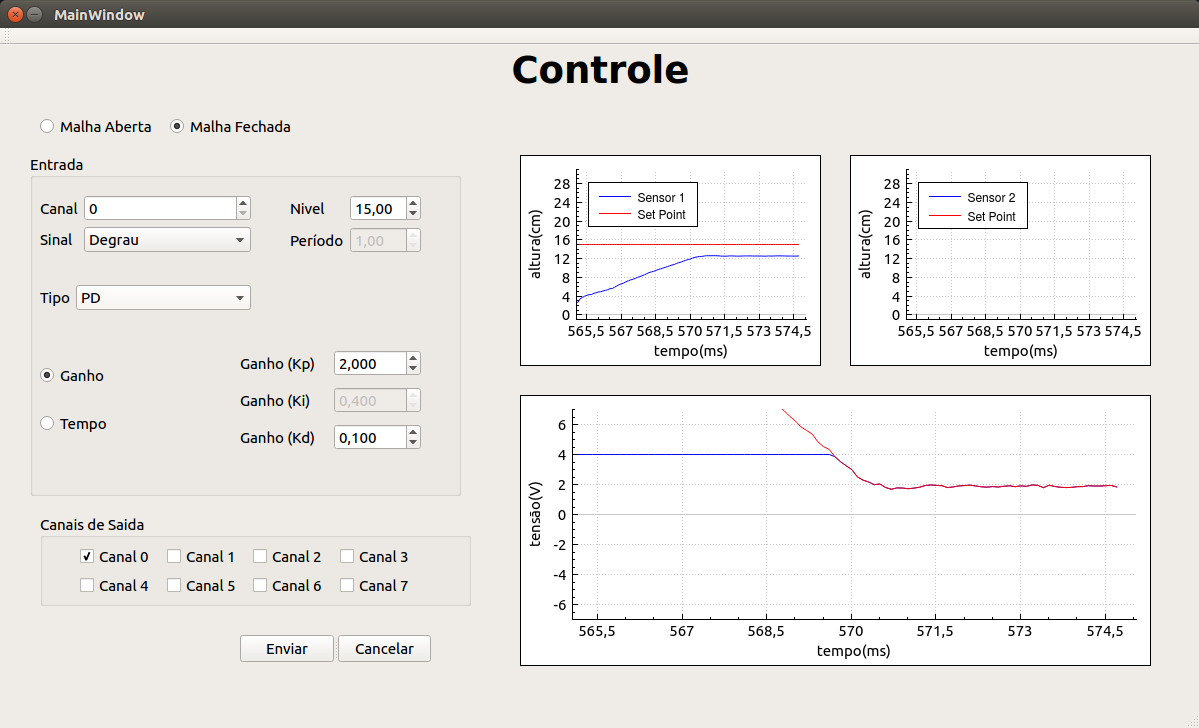
\includegraphics[width=8cm]{resultados/PD/04}\label{<figurePD5>}}\hspace{4ex}
     \subfloat[][]{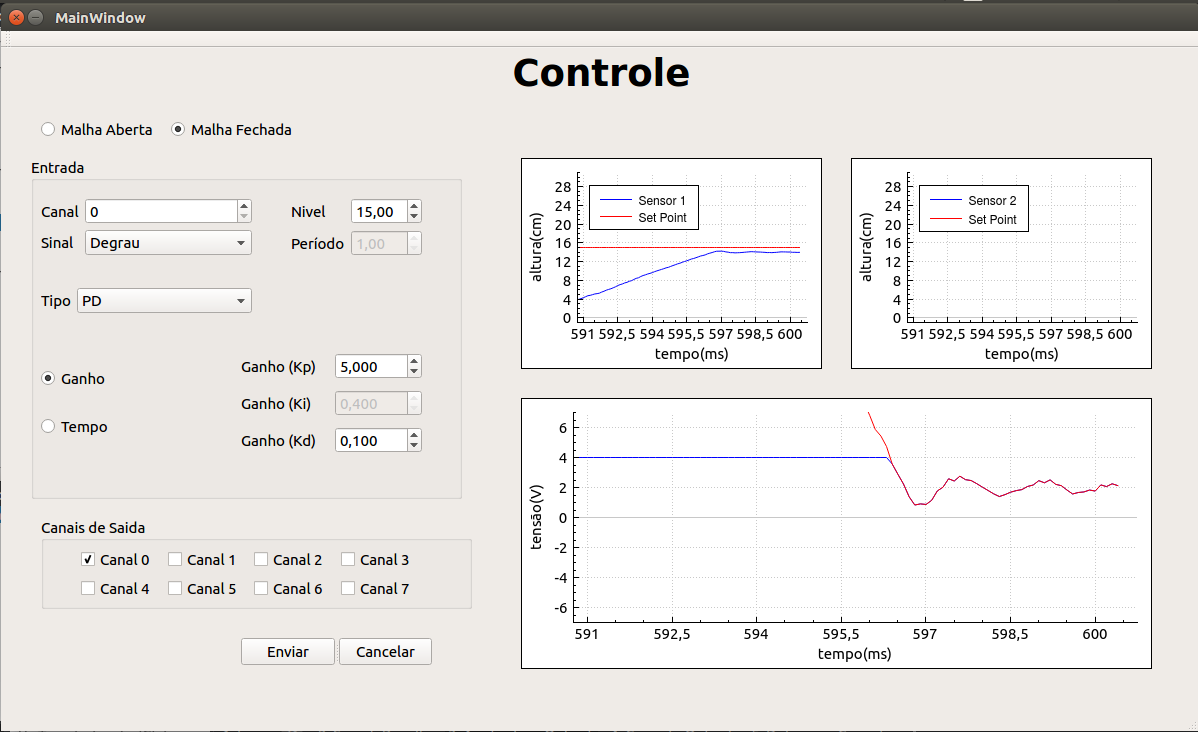
\includegraphics[width=8cm]{resultados/PD/05}\label{<figurePD6>}}\\
     \subfloat[][]{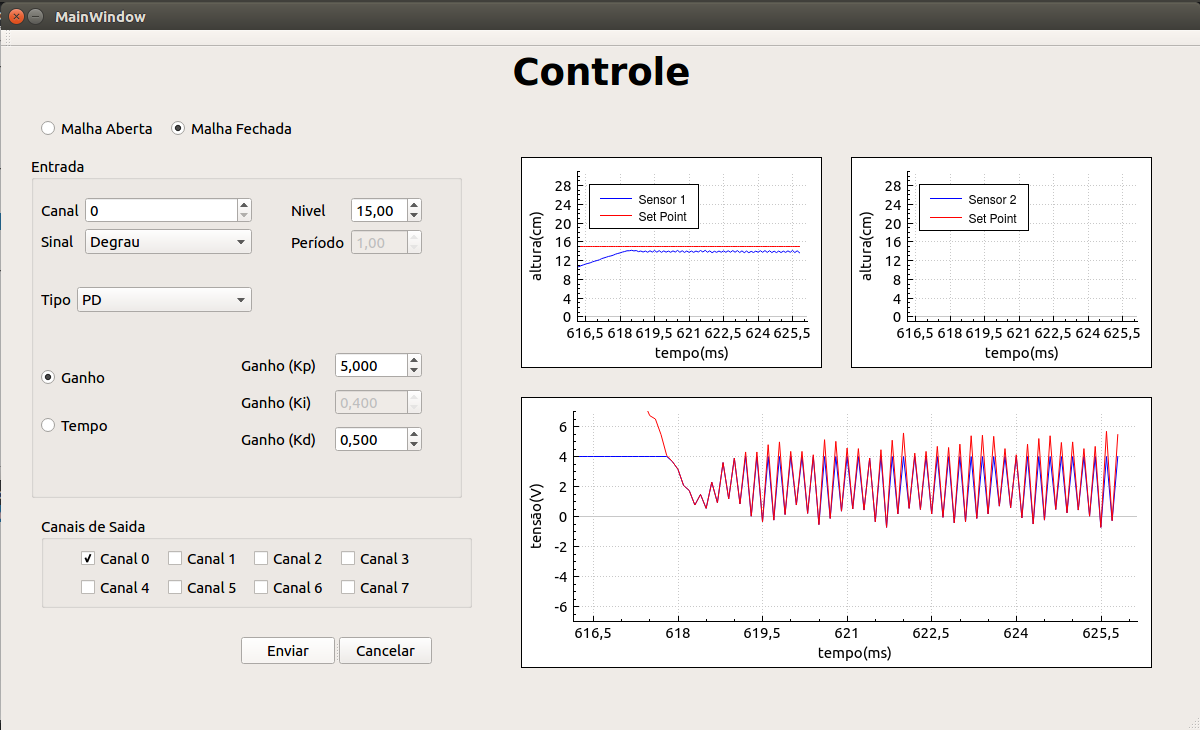
\includegraphics[width=8cm]{resultados/PD/06}\label{<figurePD7>}}
     \caption{Controle PD}
     \label{controlePD}
\end{figure}

\subsection{Controle PID}
\hspace{4ex}Usando o controlador PID é possível constatar uma diminuição do overshoot e no tempo de resposta.
\begin{figure}[H]
     \centering
     \subfloat[][]{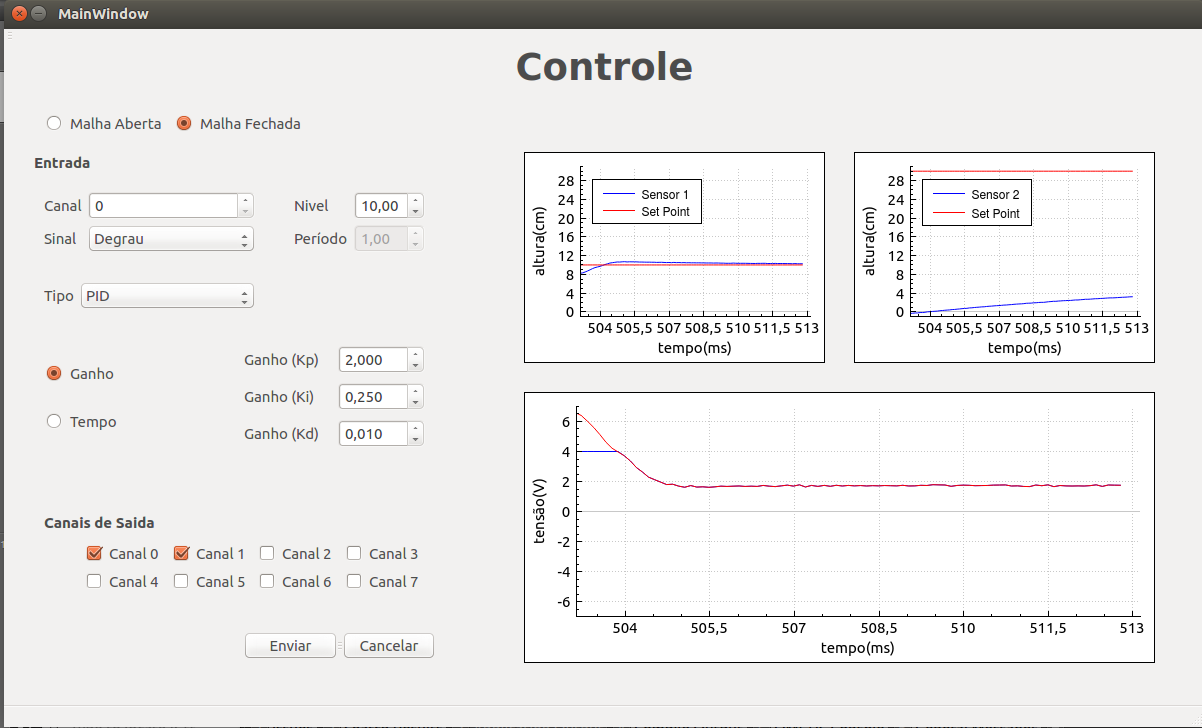
\includegraphics[width=8cm]{resultados/PID/00}\label{<figurePID1>}}\hspace{4ex}
     \subfloat[][]{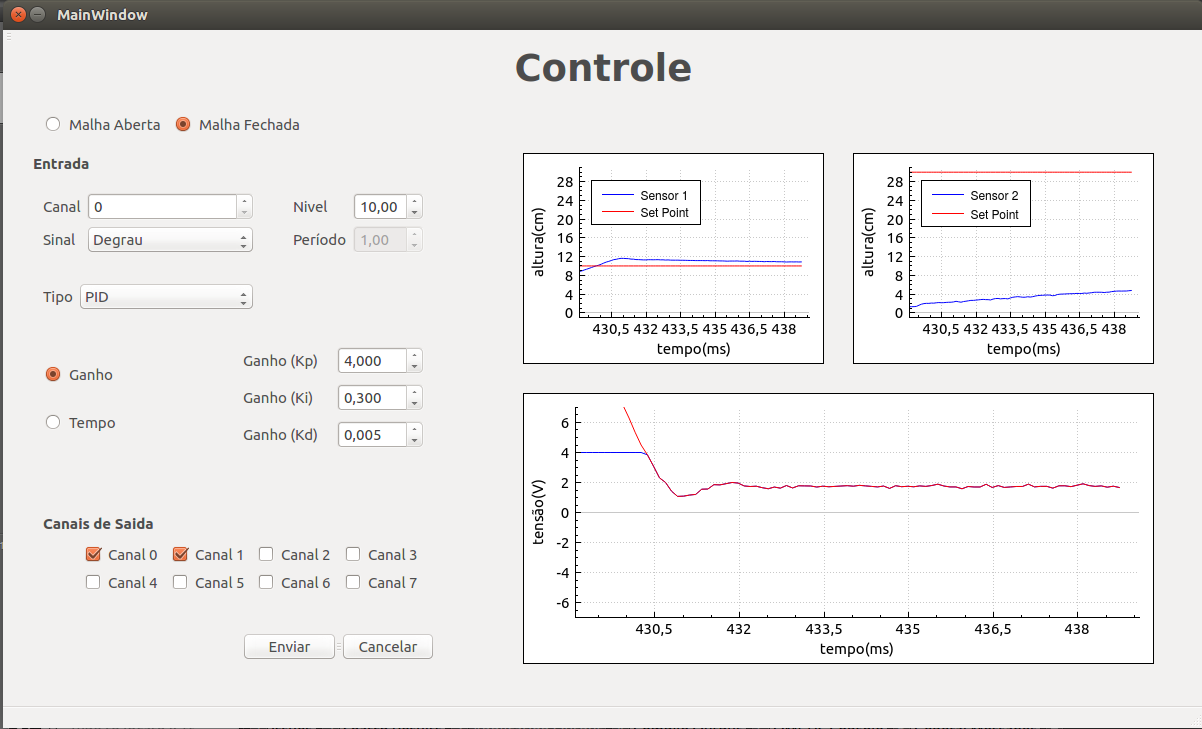
\includegraphics[width=8cm]{resultados/PID/01}\label{<figurePID2>}}\\
     \subfloat[][]{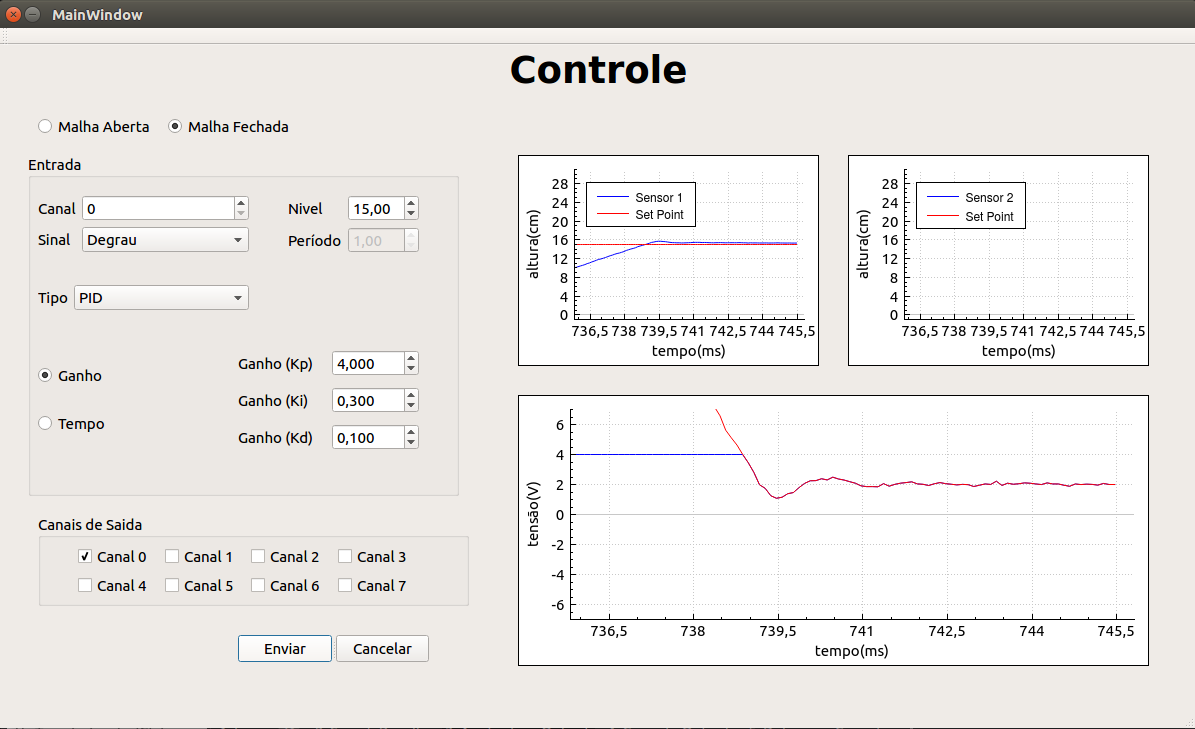
\includegraphics[width=8cm]{resultados/PID/02}\label{<figurePID3>}}\hspace{4ex}
     \subfloat[][]{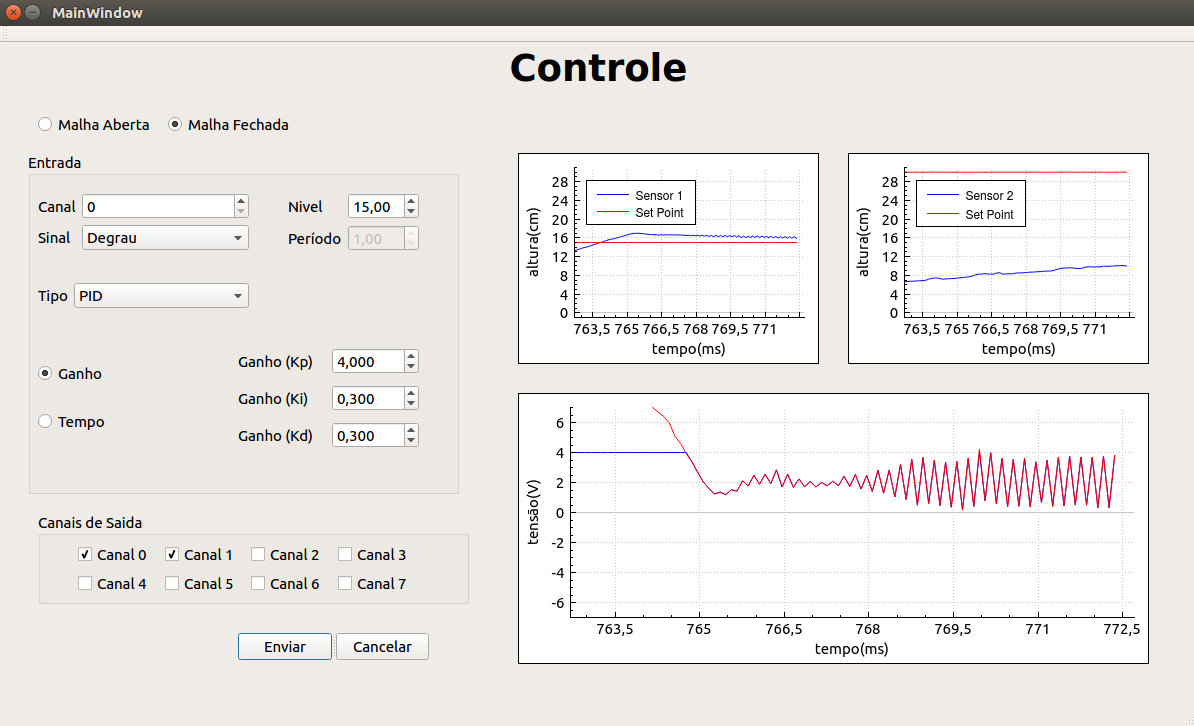
\includegraphics[width=8cm]{resultados/PID/03}\label{<figurePID4>}}\\
     \subfloat[][]{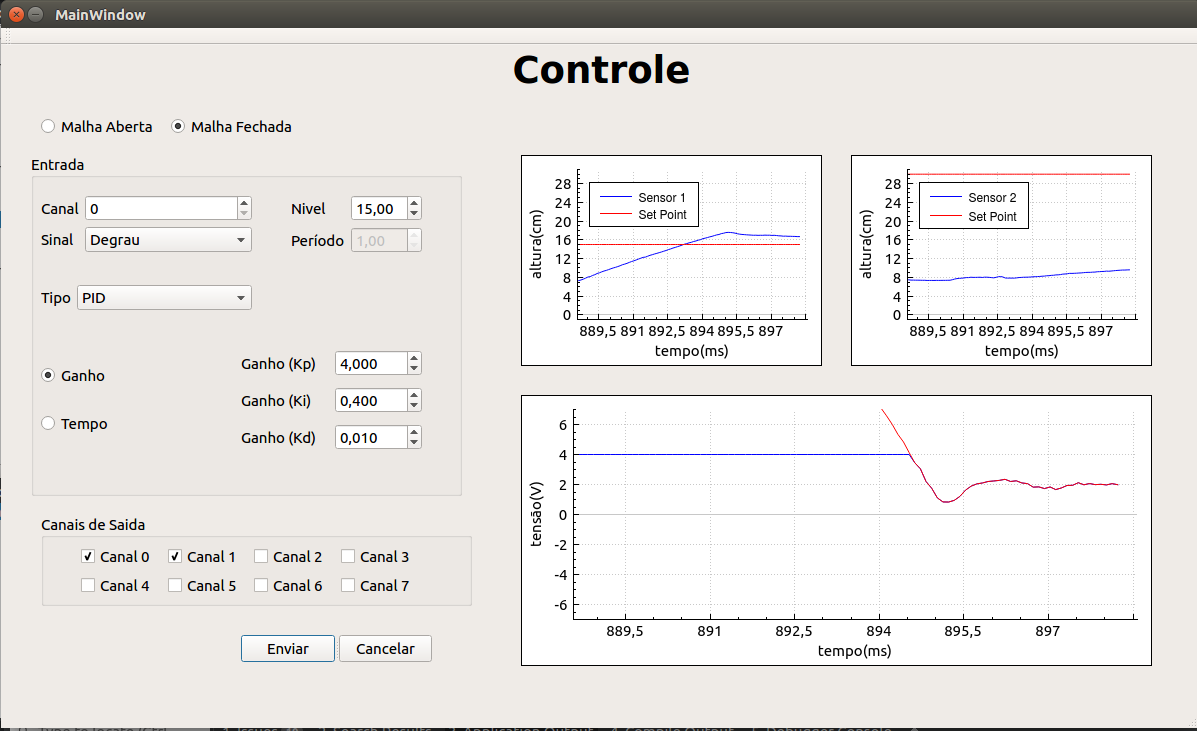
\includegraphics[width=8cm]{resultados/PID/04}\label{<figurePID5>}}\hspace{4ex}
     \subfloat[][]{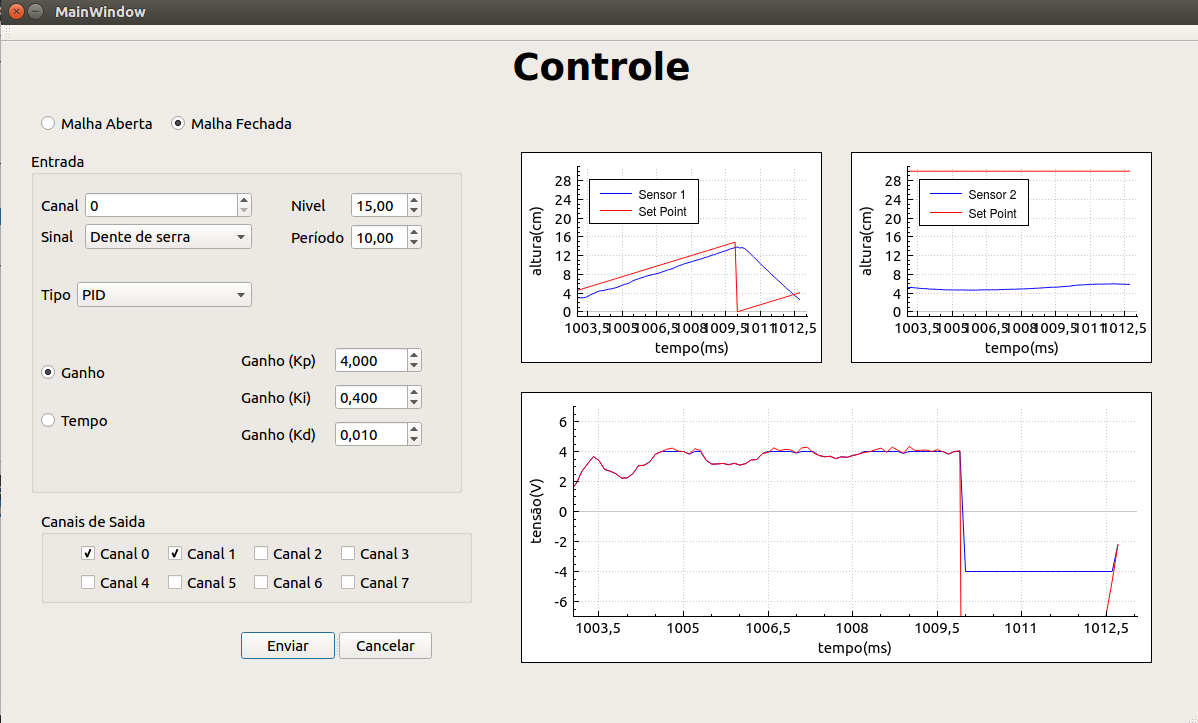
\includegraphics[width=8cm]{resultados/PID/05}\label{<figurePID6>}}\\
     \subfloat[][]{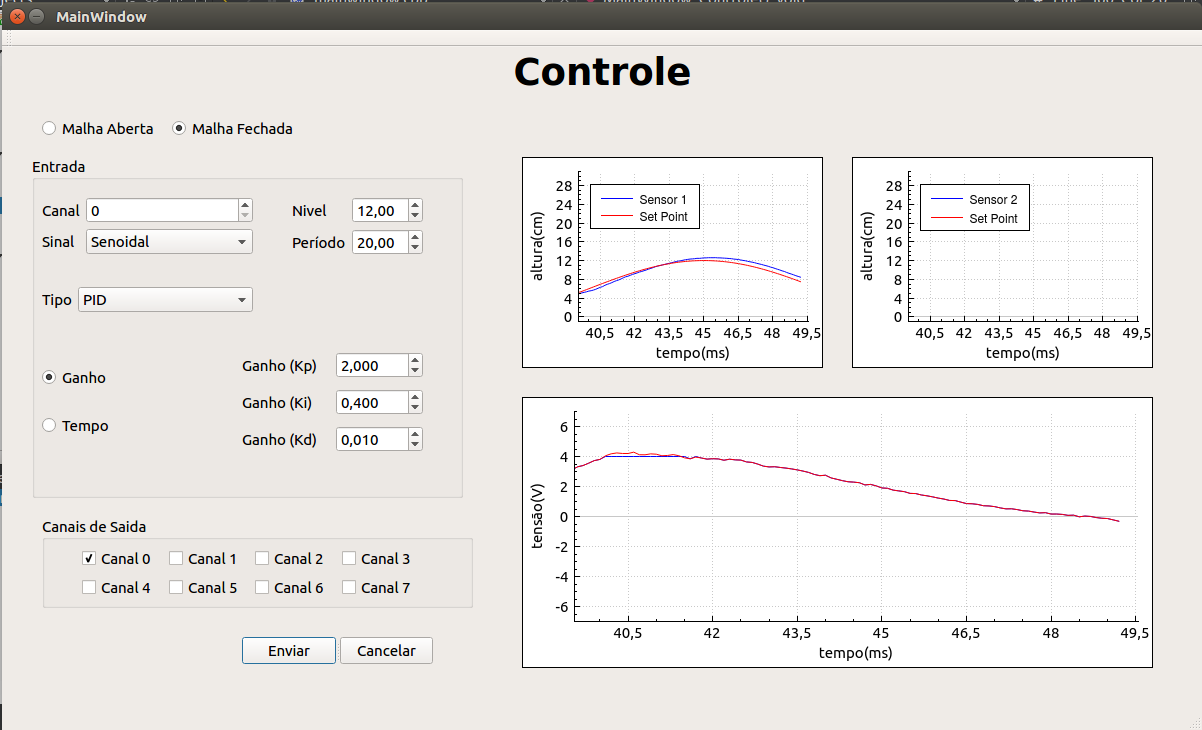
\includegraphics[width=8cm]{resultados/PID/06}\label{<figurePID7>}}
     \caption{Controle PID}
     \label{steady_state}
\end{figure}

\subsection{Controle PI-D}
\hspace{4ex}Fazendo uso do controlador PI-D é possível ver que existe menos variações bruscas no sinal de controle, além do tempo de resposta ser mais rápido, veja a figura \ref{controlePI-D}. Esse sinal parece ser melhor para sinais que possuem uma maior variancia.
\begin{figure}[H]
     \centering
     \subfloat[][]{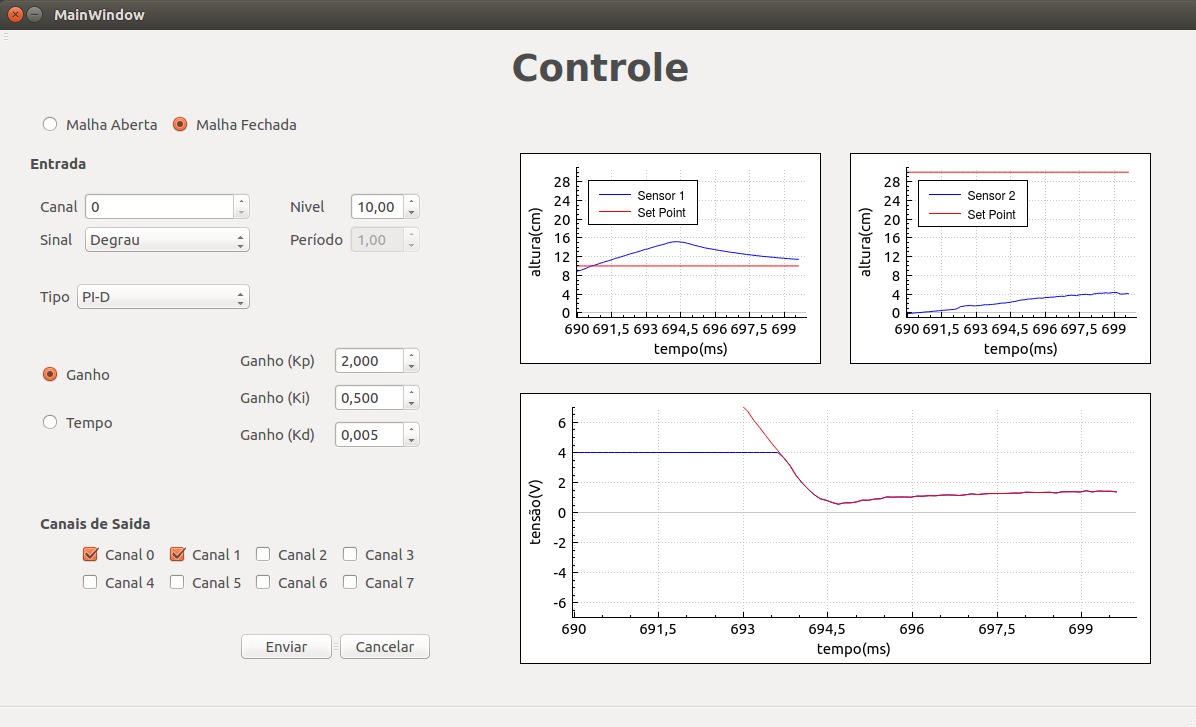
\includegraphics[width=8cm]{resultados/PI-D/00}\label{<figurePI_D1>}}\hspace{4ex}
     \subfloat[][]{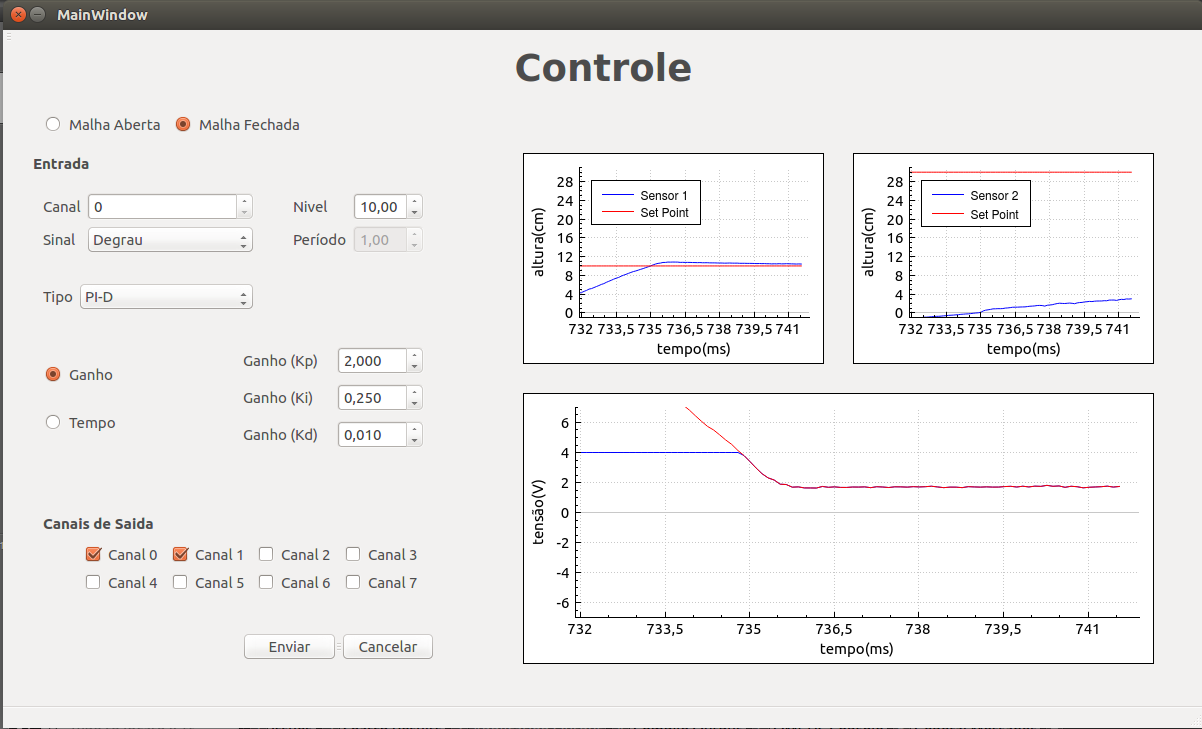
\includegraphics[width=8cm]{resultados/PI-D/01}\label{<figurePI_D2>}}\\
     \subfloat[][]{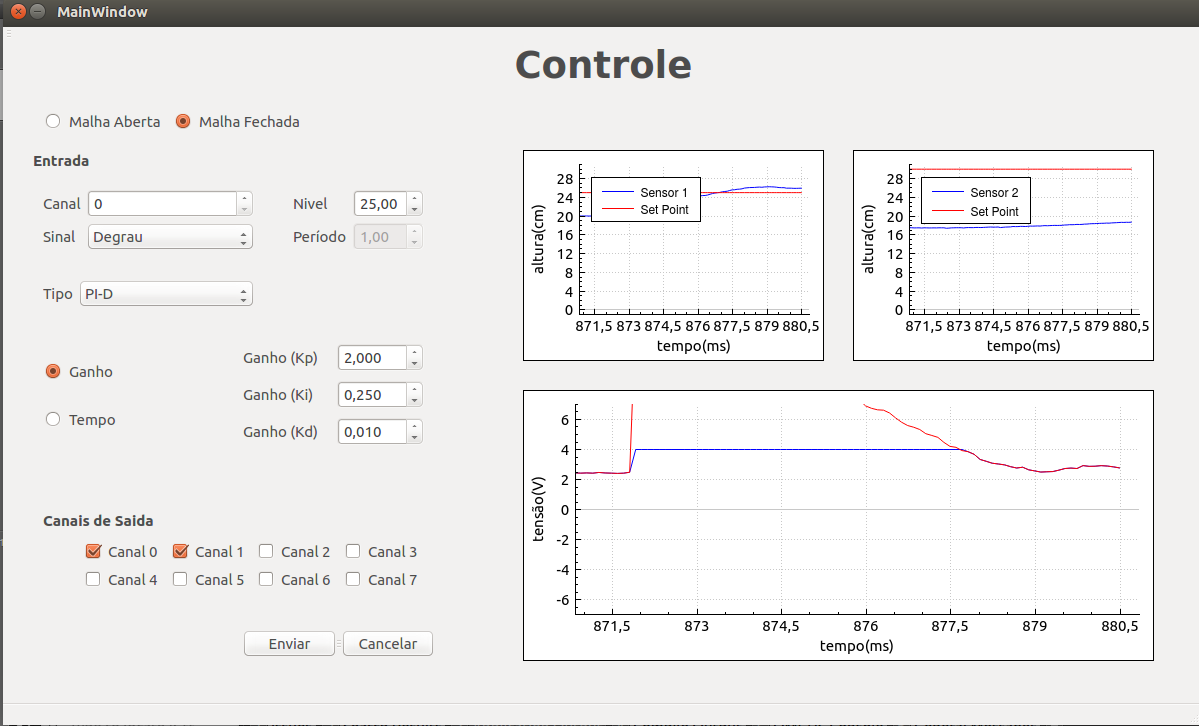
\includegraphics[width=8cm]{resultados/PI-D/02}\label{<figurePI_D3>}}\hspace{4ex}
     \subfloat[][]{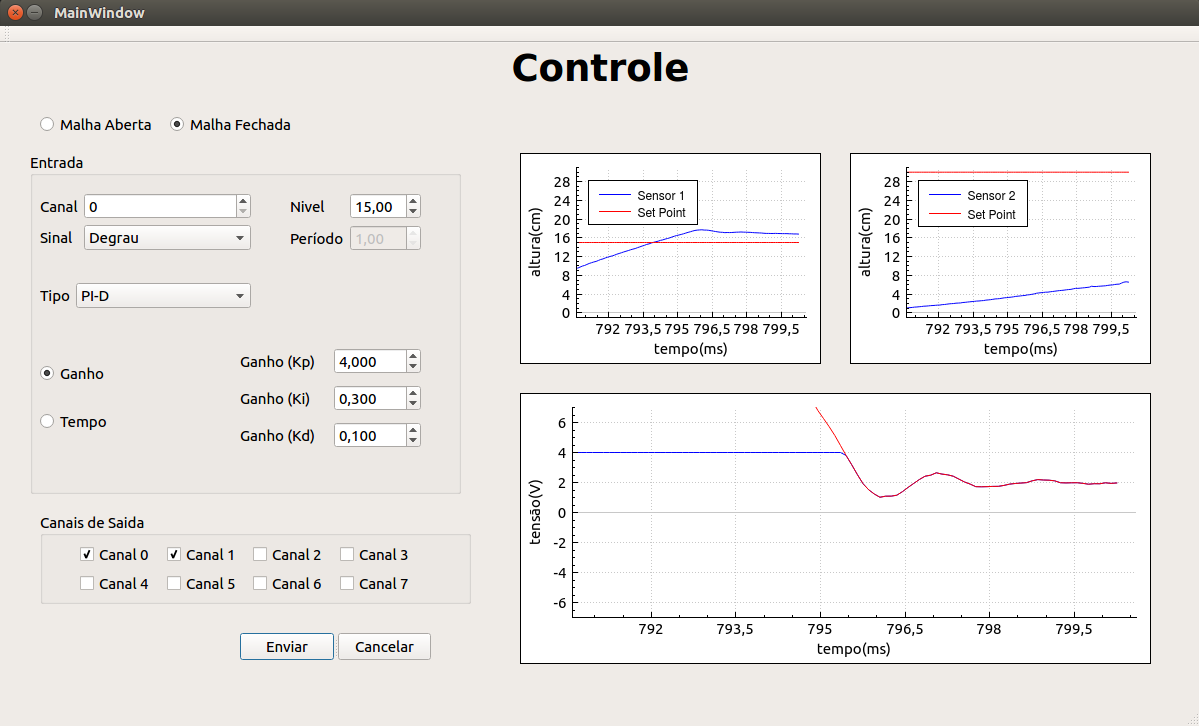
\includegraphics[width=8cm]{resultados/PI-D/03}\label{<figurePI_D4>}}\\
     \subfloat[][]{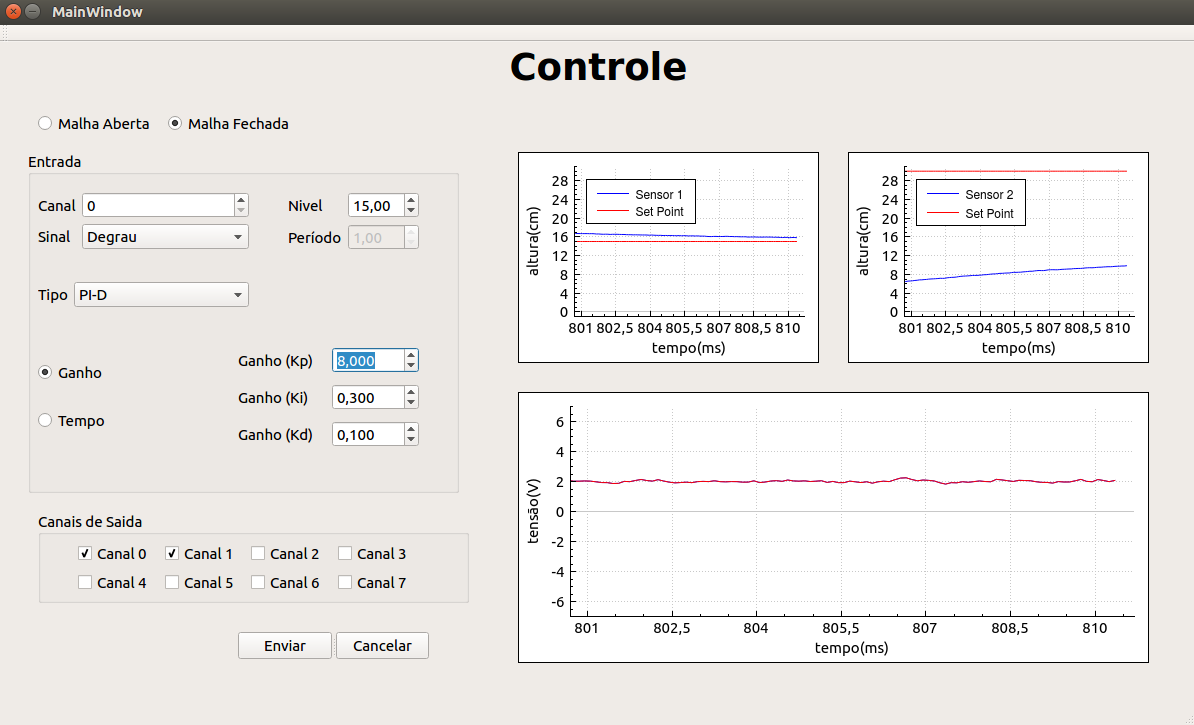
\includegraphics[width=8cm]{resultados/PI-D/04}\label{<figurePI_D5>}}\hspace{4ex}
     \subfloat[][]{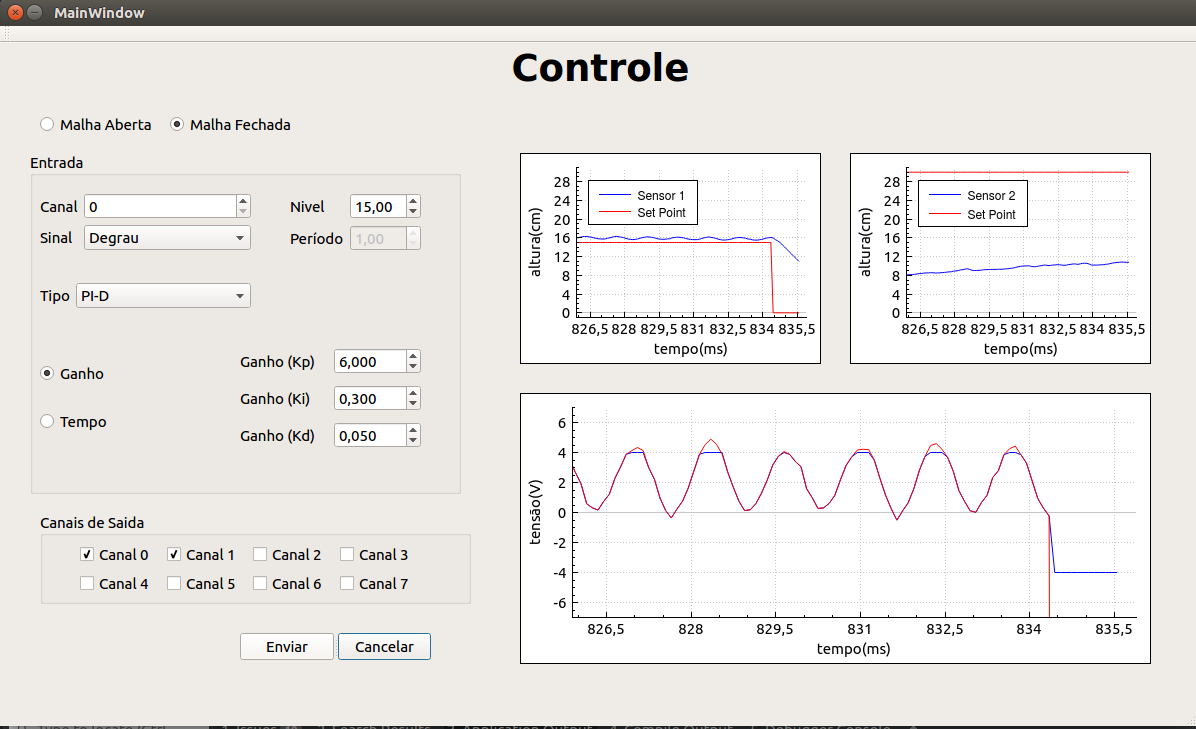
\includegraphics[width=8cm]{resultados/PI-D/05}\label{<figurePI_D6>}}\\
     \subfloat[][]{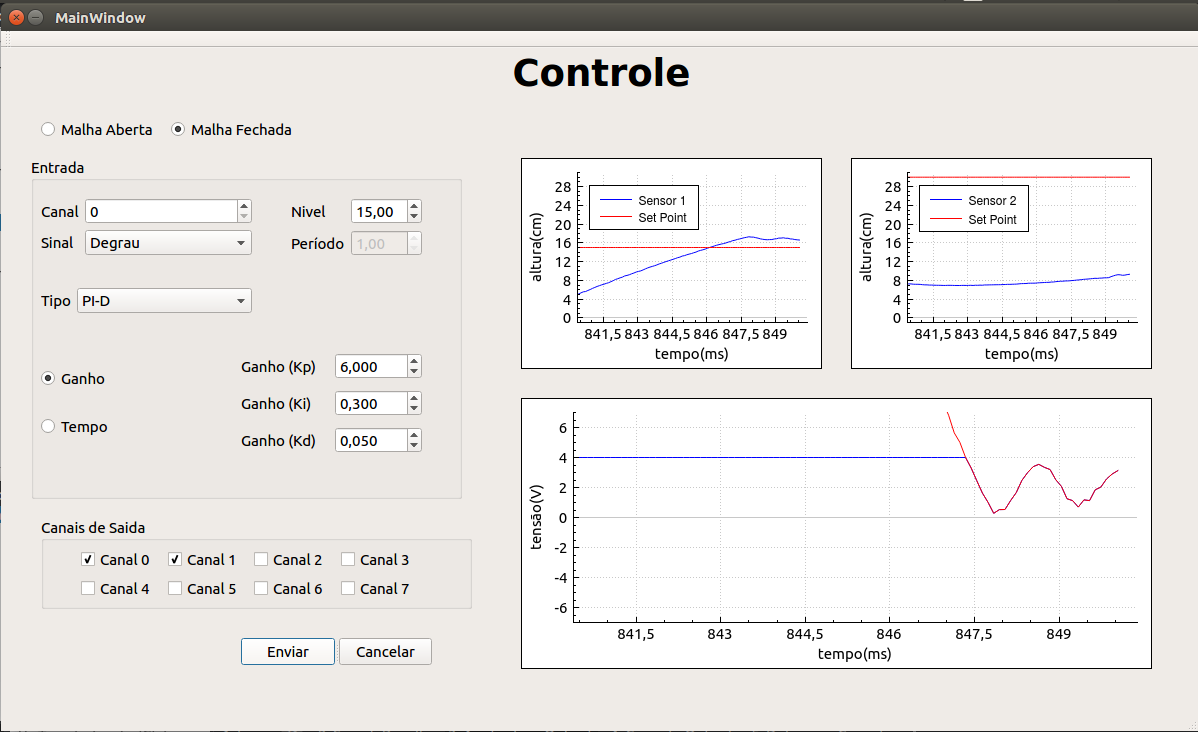
\includegraphics[width=8cm]{resultados/PI-D/06}\label{<figurePI_D7>}}\hspace{4ex}
     \subfloat[][]{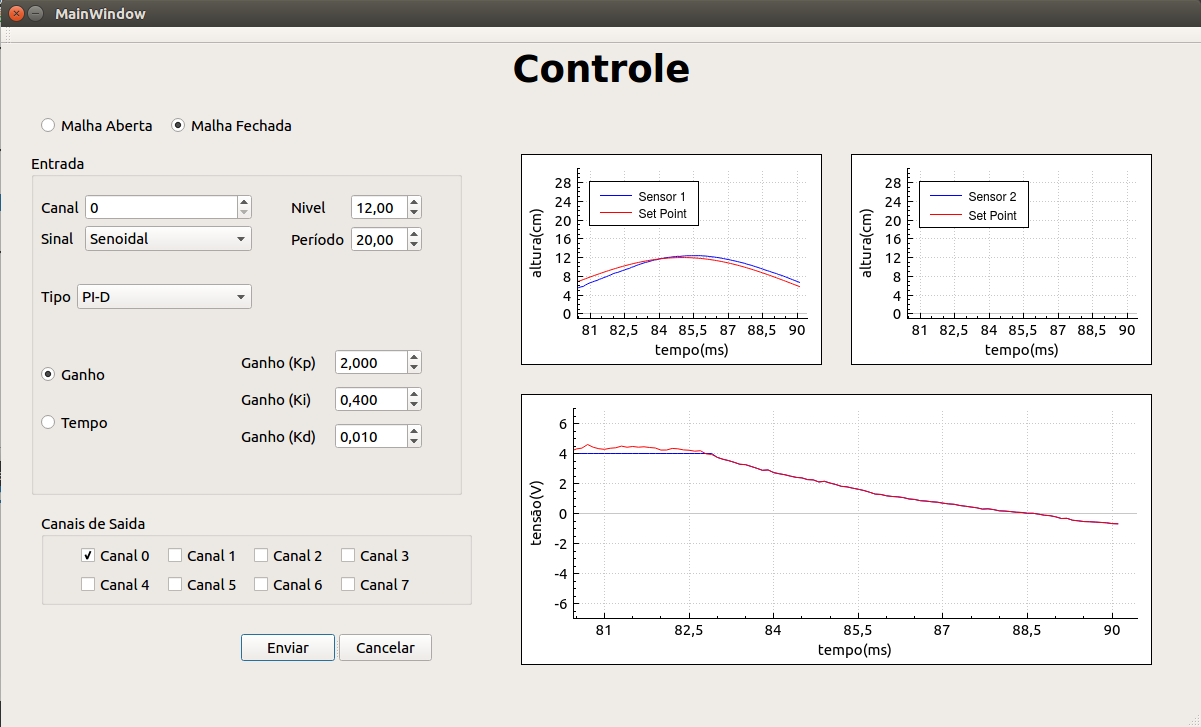
\includegraphics[width=8cm]{resultados/PI-D/07}\label{<figurePI_D8>}}
     \caption{Controle PI-D}
     \label{controlePI-D}
\end{figure}

\newpage

%%%%%%%%%% CONCLUSÃO %%%%%%%%%%%%%%%

\thispagestyle{main}

\section{CONCLUSÃO}


\hspace{4ex}Através dos testes realizados, é possível perceber a menor eficiência dos controladores P e PI na administração da resposta transitória. Por um lado, ambos melhoram a resposta em regime, com o PI apresentando erro quase zero do sinal de controle em relação ao sinal de referência, por outro, essa maior aproximação ao valor desejado vem às custas da manipulação de variáveis que podem: instabilizar o sistema – caso de Kp – ou aumentar o overshoot – caso de Ki. O controlador PD, que se mostra visivelmente melhor na resposta transitória, apresenta um maior erro na resposta em regime, e sua variável Kd pode deixar o sistema muito oscilatório.

Os controladores PID e PI-D mostraram-se capazes de produzir bons resultados tanto na resposta transitória quanto na resposta em regime: houve diminuição do overshoot, menor tempo de resposta e sinal de controle muito próximo ao sinal de referência. Os testes com o PI-D revelam também a atuação deste na redução de variações bruscas no sinal de controle. 

\newpage

%%%%%%%% REFERÊNCIAS %%%%%%%%%%%%%%%%%

\thispagestyle{empty}
\section{BIBLIOGRAFIA}
 .
 
Dorf, R.; Bishop, R. Sistemas de controle modernos. Rio de Janeiro (RJ): LTC, 2009. 

Ogata, K. Modern control engineering. Boston: Prentice Hall, 2010.


%Referências bibliogáficas (geradas automaticamente)
%\addcontentsline{toc}{chapter}{Referências bibliográficas}
%\bibliography{bib/bibliografia}

%Apêndice A
%\include{apendice}

\end{document}
